\documentclass[12pt]{article}

\usepackage{graphicx}
\usepackage{pgffor}
\usepackage{caption}
\usepackage{subfig}
\usepackage{subcaption}
\usepackage{tabularray}
\usepackage{color}
\usepackage{alltt}
\usepackage{float}
\usepackage{amsmath}
\usepackage{amsthm}
\usepackage{yhmath}
\usepackage{xcolor}
\usepackage{soul}
\usepackage{hyperref}
\usepackage{cleveref}
\usepackage{multirow}
\usepackage{pdfpages}
\usepackage{datetime}
\usepackage{makecell}
\usepackage{pdflscape}
\usepackage{array}
\usepackage{longtable}
\usepackage{booktabs}


\usepackage{bm}
\usepackage{dsfont}

% blackboard bold 
\newcommand{\ind}{\mathds{1}}
\newcommand{\R}{\mathds{R}}
\newcommand{\N}{\mathds{N}}
\newcommand{\Q}{\mathds{Q}}
\providecommand{\C}{}
\renewcommand{\C}{\mathds{C}}
\providecommand{\P}{}
\renewcommand{\P}{\mathds{P}}
\newcommand{\Z}{\mathds{Z}}
\newcommand{\E}{\mathds{E}}
\newcommand{\K}{\mathds{K}}
\renewcommand{\L}{\mathds{L}}
\newcommand{\V}{\mathds{V}}
\newcommand{\F}{\mathds{F}}
\providecommand{\G}{}
\newcommand{\D}{\mathds{D}}

% bold letters
\newcommand{\bnull}{\bm{0}}
\newcommand{\ba}{\bm{a}}
\newcommand{\bb}{\bm{b}}
\newcommand{\bc}{\bm{c}}
\newcommand{\bd}{\bm{d}}
\newcommand{\be}{\bm{e}}
% \newcommand{\bf}{\bm{f}}
\newcommand{\bg}{\bm{g}}
\newcommand{\bh}{\bm{h}}
\newcommand{\bi}{\bm{i}}
\newcommand{\bj}{\bm{j}}
\newcommand{\bk}{\bm{k}}
\newcommand{\bl}{\bm{l}}
% \newcommand{\bm}{\bm{m}}
\newcommand{\bn}{\bm{n}}
\newcommand{\bo}{\bm{o}}
\newcommand{\bp}{\bm{p}}
\newcommand{\bq}{\bm{q}}
\newcommand{\br}{\bm{r}}
\newcommand{\bs}{\bm{s}}
\newcommand{\bt}{\bm{t}}
\newcommand{\bu}{\bm{u}}
\newcommand{\bv}{\bm{v}}
\newcommand{\bw}{\bm{w}}
\newcommand{\bx}{\bm{x}}
\newcommand{\by}{\bm{y}}
\newcommand{\bz}{\bm{z}}

% bold letters
\newcommand{\bA}{\bm{A}}
\newcommand{\bB}{\bm{B}}
\newcommand{\bC}{\bm{C}}
\newcommand{\bD}{\bm{D}}
\newcommand{\bE}{\bm{E}}
% \newcommand{\bf}{\bm{f}}
\newcommand{\bG}{\bm{G}}
\newcommand{\bH}{\bm{H}}
\newcommand{\bI}{\bm{I}}
\newcommand{\bJ}{\bm{J}}
\newcommand{\bK}{\bm{K}}
\newcommand{\bL}{\bm{L}}
\newcommand{\bM}{\bm{M}}
\newcommand{\bN}{\bm{N}}
\newcommand{\bO}{\bm{O}}
\newcommand{\bP}{\bm{P}}
\newcommand{\bQ}{\bm{Q}}
\newcommand{\bR}{\bm{R}}
\newcommand{\bS}{\bm{S}}
\newcommand{\bT}{\bm{T}}
\newcommand{\bU}{\bm{U}}
\newcommand{\bV}{\bm{V}}
\newcommand{\bW}{\bm{W}}
\newcommand{\bX}{\bm{X}}
\newcommand{\bY}{\bm{Y}}
\newcommand{\hbY}{\hat{\bm{Y}}}
\newcommand{\bZ}{\bm{Z}}


% calligraphic letters
\newcommand{\Acal}{\mathcal{A}}
\newcommand{\Bcal}{\mathcal{B}}
\newcommand{\Ccal}{\mathcal{C}}
\newcommand{\Dcal}{\mathcal{D}}
\newcommand{\Ecal}{\mathcal{E}}
\newcommand{\Fcal}{\mathcal{F}}
\newcommand{\Gcal}{\mathcal{G}}
\newcommand{\Hcal}{\mathcal{H}}
\newcommand{\Ical}{\mathcal{I}}
\newcommand{\Jcal}{\mathcal{J}}
\newcommand{\Kcal}{\mathcal{K}}
\newcommand{\Lcal}{\mathcal{L}}
\newcommand{\Mcal}{\mathcal{M}}
\newcommand{\Ncal}{\mathcal{N}}
\newcommand{\Ocal}{\mathcal{O}}
\newcommand{\Pcal}{\mathcal{P}}
\newcommand{\Qcal}{\mathcal{Q}}
\newcommand{\Rcal}{\mathcal{R}}
\newcommand{\Scal}{\mathcal{S}}
\newcommand{\Tcal}{\mathcal{T}}
\newcommand{\Ucal}{\mathcal{U}}
\newcommand{\Vcal}{\mathcal{V}}
\newcommand{\Wcal}{\mathcal{W}}
\newcommand{\Xcal}{\mathcal{X}}
\newcommand{\Ycal}{\mathcal{Y}}
\newcommand{\Zcal}{\mathcal{Z}}

% greek letters
\newcommand{\eps}{\varepsilon}
\newcommand{\sd}{\sigma}
\newcommand{\ssd}{\sigma^2}
\newcommand{\gb}[1]{\beta_#1}
\newcommand{\hbe}[1]{\hat{\beta}_#1}
\newcommand{\beps}{\bm{\varepsilon}}
\newcommand{\hbeps}{\hat{\bm{\varepsilon}}}
\newcommand{\balpha}{\bm{\alpha}}
\newcommand{\bbeta}{\bm{\beta}}
\newcommand{\hbbeta}{\hat{\bm{\beta}}}
\newcommand{\bchi}{\bm{\chi}}
\newcommand{\bdelta}{\bm{\delta}}
\newcommand{\bepsilon}{\bm{\epsilon}}
\newcommand{\bphi}{\bm{\phi}}
\newcommand{\bgamma}{\bm{\gamma}}
\newcommand{\betah}{\bm{\etah}}
\newcommand{\btheta}{\bm{\theta}}
\newcommand{\htheta}{\hat{\theta}}
\newcommand{\hbtheta}{\hat{\bm{\theta}}}
\newcommand{\vtheta}{\vartheta}
\newcommand{\bvtheta}{\bm{\vartheta}}
\newcommand{\hbvtheta}{\hat{\bm{\vartheta}}}
\newcommand{\hTheta}{\hat{\Theta}}
\newcommand{\btau}{\bm{\tau}}
\newcommand{\htau}{\hat{\tau}}
\newcommand{\hbtau}{\hat{\bm{\tau}}}
\newcommand{\biota}{\bm{\iota}}
\newcommand{\bkappa}{\bm{\kappa}}
\newcommand{\blambda}{\bm{\lambda}}
\newcommand{\bmu}{\bm{\mu}}
\newcommand{\bnu}{\bm{\nu}}
\newcommand{\bomikron}{\bm{\omikron}}
\newcommand{\bpi}{\bm{\pi}}
\newcommand{\hbpi}{\hat{\bm{\pi}}}
\newcommand{\bxi}{\bm{\xi}}
\newcommand{\bzeta}{\bm{\zeta}}
\newcommand{\bomega}{\bm{\omega}}
% logic
\newcommand{\equivto}{\Leftrightarrow}
\newcommand{\quequiv}{\quad \equivto \quad}
\newcommand{\impl}{\Rightarrow}
\newcommand{\quimpl}{\quad \Rightarrow \quad}
\newcommand{\implby}{\Leftarrow}

% linear algebra
\newcommand{\tr}{\operatorname{tr}}
\newcommand{\spann}{\operatorname{span}}
\newcommand{\col}{\operatorname{col}}
\newcommand{\rang}{\operatorname{rang}}
\newcommand{\diag}{\operatorname{diag}}
\renewcommand{\vec}{\operatorname{vec}}
\newenvironment{roweqmat}[1]{\left(\array{@{}#1@{}}}{\endarray\right)}

\newcommand{\la}{\langle}
\newcommand{\ra}{\rangle}
\newcommand{\inner}[1]{\langle #1 \rangle}
\newcommand{\proj}{\operatorname{proj}}


\renewcommand{\bar}{\overline}

% statistics
\providecommand{\Pr}{}
\renewcommand{\Pr}{\mathbb{P}}
\newcommand{\var}{{\mathds{V}\mathrm{ar}}}
\newcommand{\bias}{{\operatorname{bias}}}
\newcommand{\abias}{{\mathrm{ABias}}}
\newcommand{\AMSE}{{\mathrm{AMSE}}}
\newcommand{\AMISE}{{\mathrm{AMISE}}}
\newcommand{\cov}{{\mathds{C}\mathrm{ov}}}
\newcommand{\corr}{{\mathrm{Corr}}}
\newcommand{\ov}{\overline}
\newcommand{\wh}[1]{\widehat{#1}}
\newcommand{\wt}[1]{\widetilde{#1}}
\newcommand{\tod}{\stackrel{d}{\to}}
\newcommand{\Cov}{\text{Cov}}

\newcommand{\sumin}{\sum_{i = 1}^n}
\newcommand{\sumjn}{\sum_{j = 1}^n}


\newcommand{\KL}{\operatorname{KL}}
\DeclareMathOperator*{\argmin}{arg\,min}
\DeclareMathOperator*{\argmax}{arg\,max}


\newcommand{\softmax}{\operatorname{SoftMax}}
\newcommand{\layernorm}{\operatorname{LayerNorm}}
\newcommand{\avg}{\operatorname{avg}}
\newcommand{\relu}{\operatorname{ReLu}}

% figure environment with scaling in multiples of \textwidth
\newcommand{\fig}[1][1]{
  \includegraphics[width = #1\textwidth]
}

% footnote without mark
\makeatletter
\def\blfootnote{\gdef\@thefnmark{}\@footnotetext}
\makeatother

\newcommand{\envbreak}{ \, \\[-12pt]}
\newcommand{\tw}{\textwidth}


% Sonstiges
%\newcommand*\bigcdot{\mathpalette\bigcdot@{.5}}
%\newcommand*\bigcdot@[2]{\mathbin{\vcenter{\hbox{\scalebox{#2}{$\m@th#1\bullet$}}}}}
\newcommand{\hr}{\centerline{\rule{3.5in}{1pt}}}

\definecolor{mycolor}{HTML}{3C8031}
\newcommand{\tc}[1]{\textcolor{red}{#1}}



\newcommand{\minimage}[2]{%
  \includegraphics[width=0.08\textwidth]{../figs/cifar_images_examples/#1_#2.png}%
}

\newcommand{\minimagerow}[1]{
  \minimage{#1}{0} & \minimage{#1}{1} & \minimage{#1}{2} & \minimage{#1}{3} & \minimage{#1}{4} & \minimage{#1}{5} & \minimage{#1}{6} & \minimage{#1}{7} & \minimage{#1}{8} & \minimage{#1}{9}    
}

\newcommand*{\vertbar}{\rule[-1ex]{0.5pt}{2.5ex}}
\newcommand*{\horzbar}{\rule[.5ex]{2.5ex}{0.5pt}}


\newcommand{\mytitle}{FairML and the SQF dataset}
\newcommand{\myname}{\large Juliet Fleischer}
\newcommand{\mysupervisor}{Dr. Ludwig Bothmann}

\newcommand{\thesuffix}[1]{%
  \ifnum#1=1 st%
  \else\ifnum#1=2 nd%
  \else\ifnum#1=3 rd%
  \else th%
  \fi\fi\fi}

% Manually define the date format with the ordinal suffix
\newcommand{\mydate}{%
  ~\ifcase\month\or
  January\or February\or March\or April\or May\or June\or July\or August\or
  September\or October\or November\or December\fi, \the\day\thesuffix{\day} \number\year}

\usepackage[a4paper, width = 160mm, top = 35mm, bottom = 30mm, 
bindingoffset = 0mm]{geometry}
\usepackage[utf8]{inputenc}
\usepackage{ragged2e}
\usepackage{xcolor}
% \usepackage[round, comma]{natbib}
\usepackage[backend=biber, style=authoryear]{biblatex}
\addbibresource{../literature.bib}
\usepackage{fancyhdr}
\newcommand{\changefont}{%
    \fontsize{8}{11}\selectfont
}
\hypersetup{
  colorlinks = true,
  linkcolor = black,
  urlcolor = black,
  citecolor = black}
\pagestyle{fancy}
\fancyhead{}
\fancyhead[R]{\changefont{\mytitle}}
\fancyfoot{}
\fancyfoot[R]{\thepage}
\setlength{\headheight}{14.5pt}
\setlength{\parindent}{0pt}
\interfootnotelinepenalty = 10000

% ------------------------------------------------------------------------------
% MAIN -------------------------------------------------------------------------
% ------------------------------------------------------------------------------
\IfFileExists{upquote.sty}{\usepackage{upquote}}{}
\begin{document}

% FRONT PAGE -------------------------------------------------------------------
 
\begin{titlepage}
\begin{center}
    
\LARGE
Seminar Thesis

\vspace{0.5cm}
      
\rule{\textwidth}{1.5pt}
\LARGE
\textbf{\mytitle}
\rule{\textwidth}{1.5pt}
   
\vspace{0.5cm}
      
\large
Department of Statistics \\
Ludwig-Maximilians-Universität München

\vfill

\Large
\textbf{\myname}

\vfill

\large

Munich, \mydate
      
\vfill


\includegraphics[width = 0.4\textwidth]{../figures/sigillum.png}

\vfill

\normalsize
Submitted in fulfillment of the requirements for the degree of B. Sc.
\\
Supervised by \mytitle

\end{center}
\end{titlepage}

% CONTENTS ---------------------------------------------------------------------

\pagenumbering{Roman}
\newpage
\begin{abstract}

In the first half of this paper we provide an introduction to the most common metrics and methods in fair machine learning. We then apply the theoretical concepts to the New York Stop, Question and Frisk dataset, which will showcase difficulties that come with fairness in practice. This leads us to explore the problem of selection bias and related issues. We turn our focus to studies that have worked with the SQF dataset and established interesting theoretical results: residual unfairness and bias reversal.
The main contribution of this paper lies in comparing and contrasting the different ways in which fairness has been studied for the Stop, Question, and Frisk dataset. We show that the challenges is not to identify the right approach, but rather to understand the implications and reasoning behind each method.

\end{abstract}


\newpage
\tableofcontents
\newpage


% CHAPTERS ---------------------------------------------------------------------

\pagenumbering{arabic}
    
\section{Introduction}
% \label{intro}
As algorithms are increasingly used to make decisions that affect people's lives, it is important to ensure that these decisions are fair. 
... the field of fiar machine learning. Interesting findings, recent developments, dynamic field.
limitations: unclear definitions, same datasets used over and over again.
This paper is an uncommon introduction to fairness. In "chapter ..." it provides the reader with the most common fairness metrics and methods, found in other introductions
but then in "Chapter ...." we apply them more uncommon dataset. SQF.
Since x the police in NYC is allowed to stop individuals if they have ...
Our case study will showcase difficulties that come with fairness in practice. This leads us to explore other studies that have worked with SQF data in "chapter ...". 

\section{Related Work}
Fairness in machine learning has attracted considerable attention in recent years, leading to a rich literature of definitions and evaluation frameworks. Several works provide broad overviews of these definitions. For example, \cite{verma2018} offer a comprehensive overview of the most used fairness metrics, accompanied by a case study on the Adult dataset. \cite{castelnovo2022} highlights the nuances and subtleties that come with common fairness metrics. The work of \cite{corbett-davies} and of \cite{barocas-hardt-narayanan} serves as detailed resources that offer deeper insights into common fallacies in fairML.

Beside the definition of fairness a major branch of research has concerned itself with the design of bias migitation techniques. \cite{mehrabi2022} and \cite{caton2024} provide a detailed review. Additionally, the chapter on algorithmic fairness in the \textsl{mlr3book} by \cite{mlr3_book} serves as an accessible introduction to the practical implementation of fairness metrics and methods.\par

Beyond these more general works, a number of studies from the fields fairML, Statistics, and Economics, have focused on the SQF dataset.
\cite{goel2016} use advanced statistical methods to support the claim that non-white individuals are disproportionately targeted by the New Yorker police.
\cite{Khademi2019FADMELC} examined fairness in SQF from a causal perspective. Their study supports the complexity of this topic as they arrive at divergent conclusions, depending on which of their metrics they use.\\
In the course of this paper it will become clearer that selection bias is a major concern for the SQF data. The effects of selection bias on fairness and potential ways to counteract them have been studied by \cite{Lakkaraju2017SLPEAPPU} and \cite{favier2023}.
The other studies that explicitly use SQF \cite{Badr2022DTFANSP, rambachan2016, kallus2018} will be more closely examined in the final chapter of this paper.


\section{Fairness Metrics and Methods}
\label{sec:fairness_metrics_methods}
% \section*{Definitions of Fairness in Machine Learning}
When one starts to get into the topic of fairness in machine learning, it is easy to get overwhelmed by the sheer amount of definitions and metrics that are out there. In this chapter we try to group them in an intuitive way and motivate them in the hope to bring some clarity to readers. It is helpful to group fairness metrics in the following ways.
\begin{enumerate}
    \item Group fairness vs. individual fairness
    \item observational vs. causality-based criteria
\end{enumerate}

Broadly speaking, group fairness aims to create equality between groups and individual fairness aims to create equality between two individuals within a group. Observational fairness metrics act descriptive and use the observed distribution of random variables characterizing the population of interest to assess fairness while causality-based criteria make assumptions about the causal structure of the data and base their notion of fairness on this.
On the basis of these fundamental ideas, a plethora of formalizations have emerged. Most of them concern themselves with defining fairness for a binary classification task and one binary protected attribute (PA).
The extension to a multiclass PA is the easiest. The extension to multiple sensitive attributes, on the other hand, brings challenges with it. Also, the extension from binary classification to other tasks, such as neural networks, LLMs and other models is subject of ongoing research. As this work is meant to help you start thinking about fairness in machine learning, we will limit ourselves to the binary classification case.
To bring more clarity we will illustrate the general fairness metrics already in the context of the SQF dataset.

\subsection{Group fairness}
\begin{table}
    \begin{tabular}{lll}
        \toprule
        Independence & Separation & {Sufficiency} \\
        \midrule
        $\hat{Y} \perp A$ & $\hat{Y} \perp A | Y$ & {$Y \perp A | \hat{Y}$}\\
        \bottomrule
    \end{tabular}
\end{table}

The notion of fairness underlying group metrics is that discrimination of certain groups of the population defined via the PA should be prevented. The groups metrics presented here are observational metrics. They can be separated into three main categories, independence, separation, and sufficiency. 

\subsubsection*{Independence}
Independence is in a sense the simplest group fairness metric. It requires that the prediction $\hat{Y}$ is independent of the protected attribute $A$, so $\hat{Y} \perp A$. This is fulfilled when for each group the same proportion is classified as positive by the algorithm. In other words, the positive prediction ratio (ppr) should be the same for all values of $A$. For a binary classification task with binary sensitive attribute this can be formalized as \\
\textbf{demographic parity/statistical parity}
$$P(\hat{Y} | A = a) = P(\hat{Y} | A = b)$$
This indeed seems like a simple, perhaps too simple definition of fairness, as it only looks the distribution of $\hat{Y}$ conditioned on the group membership. There are extensions of this idea, such as conditional statistical parity. This metric allows to condition on A and a set of legitimate features E. For instance, predictive parity would mean that we require equal prediction ratios between PoC and white people while conditional statistical parity requires equal prediction ratios between PoC and white people who \textit{live within the same borough of New York} (E = borough). This can be seen as a more nuanced approach, as it allows tacking additional information into account.
The other two groups of group fairness metrics, Separation and Sufficiency can both be derived from the error matrix.
\begin{center}
    \renewcommand{\arraystretch}{1.5}  % Increase row height for a more square-like appearance
    \begin{tabular}{c|c|c|}
        \hline
        & \(Y = 0\) & \(Y = 1\) \\
        \hline
        \(\hat{Y} = 0\) & TN & FN \\
        \hline
        \(\hat{Y} = 1\) & FP & TP \\
    \end{tabular}
\end{center}

\subsubsection*{Separation}
Separation requires independence between $\hat{Y}$ and $A$ conditioned on the true label $Y$, so $\hat{Y} \perp A | Y$. This means that the focus is on equal error rates between groups, which gives rise to the following list of fairness metrics:
\begin{itemize}
    \item Equal opportunity/ False negative error rate balance $$P(\hat{Y} = 0 | Y = 1, A = a) = P(\hat{Y} = 0 | Y = 1, A = b)$$ or $P(\hat{Y} = 1 | Y = 1, A = a) = P(\hat{Y} = 1 | Y = 1, A = b)$
    \item Predictive equality/ False positive error rate balance $$P(\hat{Y} = 1 | Y = 0, A = a) = P(\hat{Y} = 1 | Y = 0, A = b)$$ or \\ $P(\hat{Y} = 0 | Y = 0, A = a) = P(\hat{Y} = 0 | Y = 0, A = b)$ 
    \item Equalized odds $$P(\hat{Y} = 1 | Y = y, A = a) = P(\hat{Y} = 1 | Y = y, A = b) \forall y \in \{0, 1\}$$ 
    \item Overall accuracy equality: $$P(\hat{Y} = Y | A = a) = P(\hat{Y} = Y | A = b)$$ 
    \item Treatment equality: $$\frac{\text{FN}}{\text{FP}} \big|_{A = a} = \frac{\text{FN}}{\text{FP}} \big|_{A = b}$$
\end{itemize}

Equal opportunity requires the false negative rates, the ratio of actual positive people that were wrongly predicted as negative, to be equal between groups.
Therefore, it is also called false negative error rate balance. When there false negative rates are equal between groups, then the true positive rates between groups are also equal.
This means requiring equal false negative rates or equal true positive rates between groups results in the same effect. Predictive equality follows the same principle as equal opportunity but instead of focusing on the false negatives, it focuses on the false positives. Again, if a classifier has equal false positive rates between groups, it also has equal true negative rates.
Equalized odds combines equal opportunity and predictive equality. It requires that the false positive and true positive rates are equal between groups, and is in this sense stricter than either of them alone. \\
In itself, these error rates are detached from the context of fairness and used in general in machine learning to assess the performance of a classifier. In essence the group metrics we outlined so far do nothing other than picking a performance metrics from the confusion matrix and requiring it to be equal between two (or more) groups in the population.
This means the well-known trade-offs for example between false positive and true positive rate are also present in the fairness metrics. As more people get correctly classified as positive usually also more people get wrongly classified as positive. {\color{red}Source}
With this comes the difficulty to choose "the right" metric for the specific task. In general one can think about this in the same way as when choosing a performance metric for a binary classifier.
In setting in which a positive prediction leads to a harmful outcome, as in the SQF setting, it often makes sense to focus on minimizing the false positive rate, while a higher false negative rate is accepted as a trade-off.
This argumentation follows the idea of. The authors distinguish between punitive and assistive tasks to help choose the right fairness metric. For punitive tasks metrics that focus on false positives, such as predictive equality are more relevant. For assistive tasks, such as deciding who receives some kind of welfare, a focus on minimizing the false negative rate could be more relevant, so equal opportunity would be more suitable.

\subsubsection*{Sufficiency}
Sufficiency requires independence between $Y$ and $A$ conditioned on $\hat{Y}$, so $Y \perp A | \hat{Y}$. Intuitively this means that we want a prediction to be equally credible between groups. When a white person gets a positive prediction the probability that it is correct should be they same as for a black person. This leads to the following fairness metrics:
\begin{itemize}
    \item Predictive parity/ outcome test requires that the probability of actually being positive, given a positive prediction is the same between groups. $$P(Y = 1 | \hat{Y} = 1, A = a) = P(Y = 1 | \hat{Y} = 1, A = b)$$
    \item Equal true negative rate follows the same principle as predictive parity. It requires that the probability of actually being negative, given a negative prediction is the same between groups.: $$P(Y = 0 | \hat{Y} = 0, A = a) = P(Y = 0 | \hat{Y} = 0, A = b)$$
    \item If we instead look at errors again, we can require equal false omission rates: $$P(Y = 1 | \hat{Y} = 0, A = a) = P(Y = 1 | \hat{Y} = 0, A = b)$$
    \item Or equal false discovery rate: $$P(Y = 0 | \hat{Y} = 1, A = a) = P(Y = 0 | \hat{Y} = 1, A = b)$$ 
    \item Conditional use accuracy equality: $$P(Y = 1 | \hat{Y} = 1, A = a) = P(Y = 1 | \hat{Y} = 1, A = b) \land P(Y = 0 | \hat{Y} = 0, A = a) = P(Y = 0 | \hat{Y} = 0, A = b)$$
\end{itemize}

False omission describes the case in which an actual positive person is predicted as negative and can be highly relevant in assistive settings, such as description of a medical treatment. False discovery rate describes the case in which an actual negative person is predicted as positive. This should be taken into account in punitive settings, in which we do not want to convict innocent people.
Just as for equalized odds as Separation metric, we can build a stronger Sufficiency metric requiring multiple conditions to hold simultaneously, e.g. conditional use accuracy equality.
Hopefully, the pattern becomes clear now. While it is easy to get overwhelmed by the amount of definitions at first, taking a closer look, it becomes clear that they are constructed in a structured way. In fact, equal false omission rate and equal false discovery rate were not introduced in the paper \cite{verma2018} but are implemented in \texttt{mlr3fairness}, and it is clear that they follow the same pattern as the other metrics.

Most (binary) classifiers work with predictions scores and a hard label classifier is applied only afterwards in form of a threshold criterion. It should therefore come as no surprise that instead of formulating fairness with $\hat{Y}$ there exist fairness metrics that use the score $S$, which typically represents the probability of belonging to the positive class. Instead of conditioning on $\hat{Y}$ as Separation metrics, we can simply condition on $S$ and define: \\
Calibration: $$P(Y = 1 | S = s, A = a) = P(Y = 1 | S = s, A = b)$$
Calibration requires that the probability for actually being positive, given a score $s$ is the same between groups. So the idea is a more fine-grained version of predictive parity. As the score can usually take values from the whole real number line, this can in practice be implemented by binning the scores \cite{verma2018}.

To compare the group fairness criteria, sufficiency takes the perspective of the decision-making instance, as usually only the prediction is known to them in the moment of decision. For example, the police, who do not yet know the true label at the time when they are supposed to decide whether someone would become a criminal.
As separation criteria condition on the true label Y it is suitable when we can be sure that $Y$ is free from any bias, so to say when $Y$ was generated via an objectively true process (this will become clearer in the chapter on bias).
Independence is best, when we want to enforce a form of equality between groups, regardless of context or any potential personal merit. While this seems to be useful in cases in which the data contains complex bias, it is unclear whether these enforcements have the intended benefits, especially over the long term. {\color{red}{Reference?}}.
It is good to understand the difference in perspectives each of the group fairness metrics take, because many of them cannot be satisfied simultaneously. This is known as the impossibility theorem \cite{hardt2016}. This means one has to decide on either Independence, Separation or Sufficiency and the choice should fit the context of the data and the decision-making process. Lastly, we note that these are not all the group fairness metrics that exist, but broadly speaking other metrics are variations of the presented ones. Some more metrics are listed in the appendix.

\subsection{Individual fairness}
If we want to equalize e.g. the false positive rates between two groups and currently group a has a higher false positive rate than group b, this would lead us to lowering the prediction threshold for b, such that more actual negative people would get classified as positive. Or if we would need to set a higher threshold for group a, such that it becomes harder for them to be classified as positive. Depending on the context, either option can seem unfair. So by trying to equalize a given metric between groups, it can happen that individuals within a group are treated unequally. Individual metrics therefore shift the focus. The underlying idea of fairness is that similar individuals should be treated similarly.
\subsubsection*{Fairness through awareness (FTA)}
FTA formalizes this idea as Lipschitz criterion. $$d_Y(\hat{y_i}, \hat{y_j}) \leq \lambda {d_X}(x_i, x_j)$$
$d_Y$ is a distance metric in the prediction space, $d_X$ is a distance metric in the feature space and $\lambda$ is a constant.
The criterion puts an upper bound to the distance between predictions of two individuals, which depends on the features of them. In other words, if two people are close in the feature space, they also should be close in the prediction space. The challenge of FTA is the definition of the equality in the feature space. \cite{castelnovo2022} states "defining when two individuals are similar is not much different from defining fairness in the first place".
In the SQF context, it could make sense to define similar individuals based on yearly income, age and neighbourhood.
Yet one could easily argue that taking the criminal history into account is important as well. After the decision for a legitimate set of features has been made, the next challenge is to choose a distance metric that appropriately captures the conceptual definition of similarity defined via the selected features.
FTA does not have one clear solution and requires domain knowledge and the choice of $d_X$ should take context-specific information into account.

\subsection*{Fairness through unawareness (FTU) or blinding}
In contrast to FTA, blinding should give a simple, context-independent rule. It tells us to not use the protected attribute explicitly in the decision-making process. When training a classifier this means discarding the PA during training.
Since FTU is a more procedural rule than a mathematical definition, there exist multiple ways to test whether the blinding worked for a classifier. One approach is to simulate a doppelgänger for each observation in the dataset. This doppelgänger has the exact same features except the protected attribute, which is flipped.
If both these instances have the same prediction, the algorithm would satisfy FTU \cite{verma2018}. \footnote{This can be seen as a from of FTA, in which we chose the distance metric to measure a distance of zero only if two people are the same on all their features except for the protected attribute. In this special case FTA and FTU are measured in the same way.} Other ways to assess FTU can be found in \cite{verma2018}. 
A problem blinding has been proxies. These are variables that are strongly correlated with the sensitive attribute. It is not enough to simply mask the information of the sensitive attribute during training because discrimination can persist via these proxies.
For SQF this would mean that we remove the race attribute during training.
A person's ethnicity, however, is strongly correlated with their place of residence. Thus, indirect discrimination based on ethnicity remains, even though the information was not directly available during training. \textbf{Suppression} extends the idea of blinding and the goal is to develop a model that is blind to not only the sensitive attribute but also the proxies. The drawback is, that it is unclear when a feature is sufficiently high correlated with the sensitive attribute to be counted as proxy. Additionally, we could lose important information by removing too many features \cite{castelnovo2022}.

\subsection{Causality-based fairness metrics}
In contrast to observational fairness metrics, causality-based notions ask whether the sensitive attribute was the \textit{reason} for the decision. If a certain (harmful) decision was made \textit{because of} the value of the sensitive attribute of a person, we deem the algorithm as unfair.
% There are causality-based concepts that focus on group-level fairness and also some that focus on individual-level fairness. We want to give an intoduction to all of them, but since this category requires a new theory we will not get into great detail.

\textbf{Group-level}: FACE, FACT (on average or on conditional average level) \parencite{Zafar2017PPNFC}\\
\textbf{Individual-level}: counterfactual fairness, path-based fairness \parencite{kusner} 
The two most common individual fairness metrics are counterfactual fairness and path-based fairness.


\subsection{Comparison and Summary}

The difference between observational and causal clear, really different approach. The division in group and individual fairness metric actually more of a nuanced differentiation. The observational metrics can rather be ordered on a plane, depending on how much information of the situation via other features X they allow.
Traditional group metrics like demographic parity, equal error rate metrics and sufficiency metrics only work with the distribution of $Y, \hat{Y}, X, A$. The individual fairness metrics take more information of the non-sensitive feature into account in order to define similarity. Metrics such as conditional demographic parity lie in between, as we allow for a relevant subset of non. Sensitive feature to be part of the definition.
\cite{castelnovo2022} therefore depict this as a plane.
The amount of approaches to measure fairness shows the complexity of the topic. There is not \textit{the} right fairness metric to choose, but there can be the best one depending on the context and the data. The next section will present ways to digitate algorithmic bias once detected by one of the fairness metrics.



\subsection{Fairness methods}
Another question fair machine learning deals with is how algorithms can be adjusted so that they fulfil one of the above fairness metrics.
Depending on when they take place in the machine learning pipeline, we distinguish between
\begin{enumerate}
    \item Pre-processing methods
    \item In-processing methods
    \item Post-processing methods
\end{enumerate}
Pre-processing methods follow the idea that the data should be modified before training, so that the algorithm learns on "corrected" data. Reweighing observations before training is an example for a preprocessing method. The idea is to assign different weights to the observations based on relative frequencies, so that the algorithm learns on a balanced dataset \cite{caton2024}.\\
In-Processing methods modify the optimization criterion, such that it also accounts for a chosen fairness metric. Introducing a regularization term to the loss function is one example of such modifications.\\
Post-processing methods work with black box algorithms, just like preprocessing methods. We only need the predictions from the model to adjust them so that again a chosen fairness metric is fulfilled. One example for this is thresholding, where we set group specific thresholds to re-classify the data after training (\cite{hardt2016}).
Depending on the task (regression, classification) and the model there are highly specified and advanced methods. For the case study in chapter 3, we limit ourselves to methods from the \texttt{mlr3fairness} package.
% mlr3fairness currently has two preprocessing methods, one postprocessing method and several fairness adjusted models implemented. We decide to use a reweighing methods that works with assigning weights to the observations to equalise the distribution of $P(Y|PA)$.
% The inprocessing method is a fairness-adjusted logistic regression implemented in mlr3fairness inspired by Zafar et. al. This method optimises for statistical parity (independence). The postprocessing method we choose aims for equalised odds and it works by randomly flipping a subset of predictions with pre-computed probabilities in order to satisfy equalised odds constraints.

\subsection{Bias and the feedback loop}
Before the application on real data, to introduce different types of biases and the context in which the ADM is embedded.
Used to assist decision-making, the machine learning model influences if someone gets admitted to college, receives a loan or is released from prison.
The circumstances of a decision are made measurable by collecting data. The algorithm learns from this data to make an optimal prediction, on which the decision-makers base their judgement on. This decision will shape the reality, which reflects in new data. This means the algorithm does not exist in isolation, but depends on the data and shapes the user's actions.\\ 
\cite{mehrabi2022} call this the data, algorithm, and user interaction feedback loop. At each stage, bias can be introduced into the process. More dangerous, bias can even be amplified as the algorithm influences decision-making on a large scale.
Consequently, every fairness project comes with the responsibility to understand the data-generating process and gain clarity on how the algorithm will be deployed in the real-world.\\
The data, algorithm, and user interaction feedback loop also helps in distinguish between various types of bias. \autoref{fig:bias_loop} depicts one exemplary type of bias for each stage of the feedback loop. It can be crucial to think about which type of bias might be relevant in a given situation as this should influence the definition of fairness and the choice of fairness adjustments. This will also become evident as we examine the SQF dataset.

\begin{figure}
    \centering
    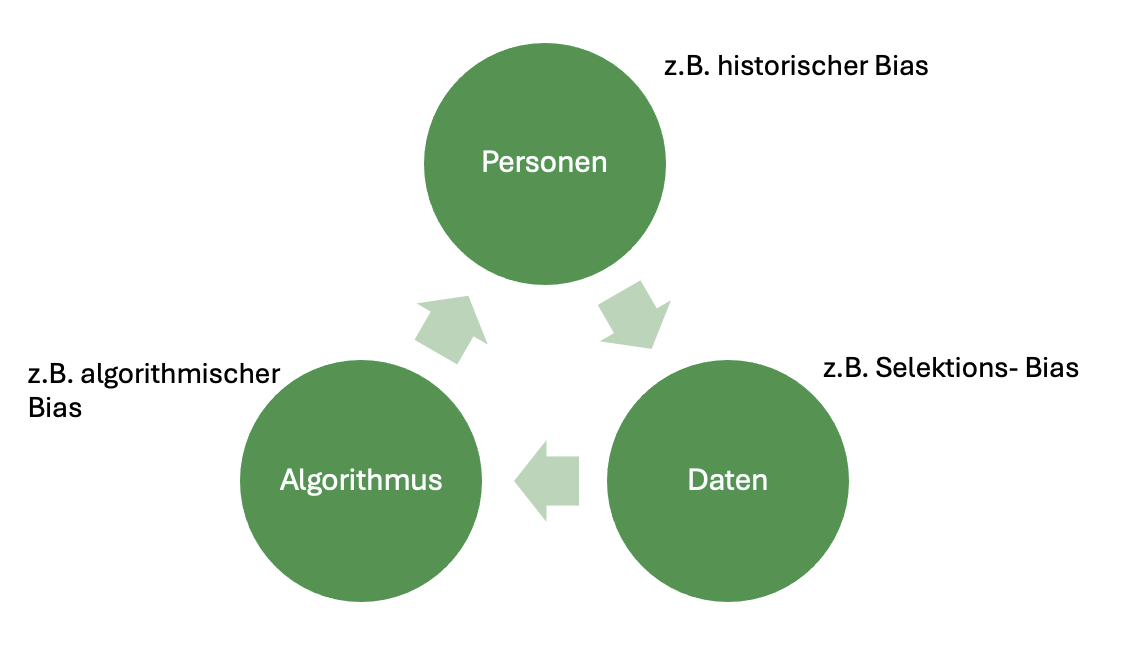
\includegraphics[width=0.7\textwidth]{../figures/bias_loop.png}
    \caption{The bias loop.}
    \label{fig:bias_loop}
\end{figure}

% \subsection*{Bias}
% We want to end this general introduction into fair machine learning by outlining the context in which the algorithm is usually embedded. On this note we also advice practitioners to think about the source of bias that could be present in your situation, as this \textit{should} influence how fairness is defined and what fairness adjustments are appropriate. This will motivate the potential difficulties that can arise when implementing fairness in the real world.
% \cite{caton2024} describe the situation as follows. The algorithm is embedded in a feedback loop with the user and data.
% We as a society make decision, which reflect our reality. We make our reality measurable by collecting data. The algorithm learns from this data and makes predictions, on which we base new decisions. 
% At each of these three points bias can be introduced into the process and, above all, bias can also be reinforced in the course of this process.
% In the context of the Stop, Question, and Frisk data, historical bias and selection bias are probably the most relevant sources of bias.
% Historical bias can shows itself in different ways. In our case it would mean that we assume that some people in our data have repeatedly experienced discrimination in terms of being arrested.
% Selection bias refers to the fact that the data is not representative of the population of New York City, because the decision to stop someone is based on a biased decision policy.




\section{Case Study: Stop, Question, and Frisk}
\label{sec:case_study}
% \subsection*{Fairness Experiment: Stop, Question, and Frisk data}
After introducing the theoretical tools for assessing fairness, we turn to a case study on the stop-and-frisk practice. A police officer is allowed to stop a person if they have reasonable suspicion that the person has committed, is committing, or is about to commit a crime.
During the stop the officer is allowed to frisk a person (pat-down the person's outer clothing) or search them more carefully.
The stop can result in a summon, an arrest or no further consequences. After a stop was made, the officer is required to fill out a form, documenting the stop. This data is published yearly by the NYPD.
As mentioned in the introduction the so-called "New York strategy" \cite{gelman2007} is highly controversial. The aggressive way in whcih the stop-and-frisk practice was being implemented during 2004 to 2012 in NYC was indeed deemed unconstitutional in 2013, violating the fourth and fourteenth amendment {\color{red} Source}


\subsection{Fairness Experiment: Setup}
For our analysis the task is to predict the arrest of a suspect. We compare the following models in terms of fairness and model performance, measured by the difference in true positive rates and the classification accuracy respectively.:
\begin{itemize}
    \item Regular Random Forest
    \item Reweighing to balance disparate impact metric (Pre-Processing)
    \item Classification Fair Logistic Regression With Covariance Constraints Learner (In-Processing)
    \item Equalized Odds Debiasing (Post-Processing)
\end{itemize}
More details about the methods can be found in the \texttt{mlr3} documentation \cite{mlr3_book}.  
For reweighing, see \href{https://mlr3fairness.mlr-org.com/reference/mlr_pipeops_reweighing.html}{mlr3fairness Reweighing}.  
For fair logistic regression, refer to \href{https://rdrr.io/cran/mlr3fairness/man/mlr_learners_classif.fairzlrm.html}{Fair Logistic Regression}.  
For equalized odds, check \href{https://mlr3fairness.mlr-org.com/reference/mlr_pipeops_equalized_odds.html}{Equalized Odds}.  

% Reweighing: https://mlr3fairness.mlr-org.com/reference/mlr_pipeops_reweighing.html
% Fair logistic regression: https://rdrr.io/cran/mlr3fairness/man/mlr_learners_classif.fairzlrm.html
% EOd: https://mlr3fairness.mlr-org.com/reference/mlr_pipeops_equalized_odds.html
% mlr3book: https://mlr3book.mlr-org.com/chapters/chapter14/algorithmic_fairness.html
% https://mlr3fairness.mlr-org.com/#debiasing-methods

\subsection{Data description}
\begin{figure}
  \centering
  \begin{minipage}{0.49\textwidth}
      \centering
      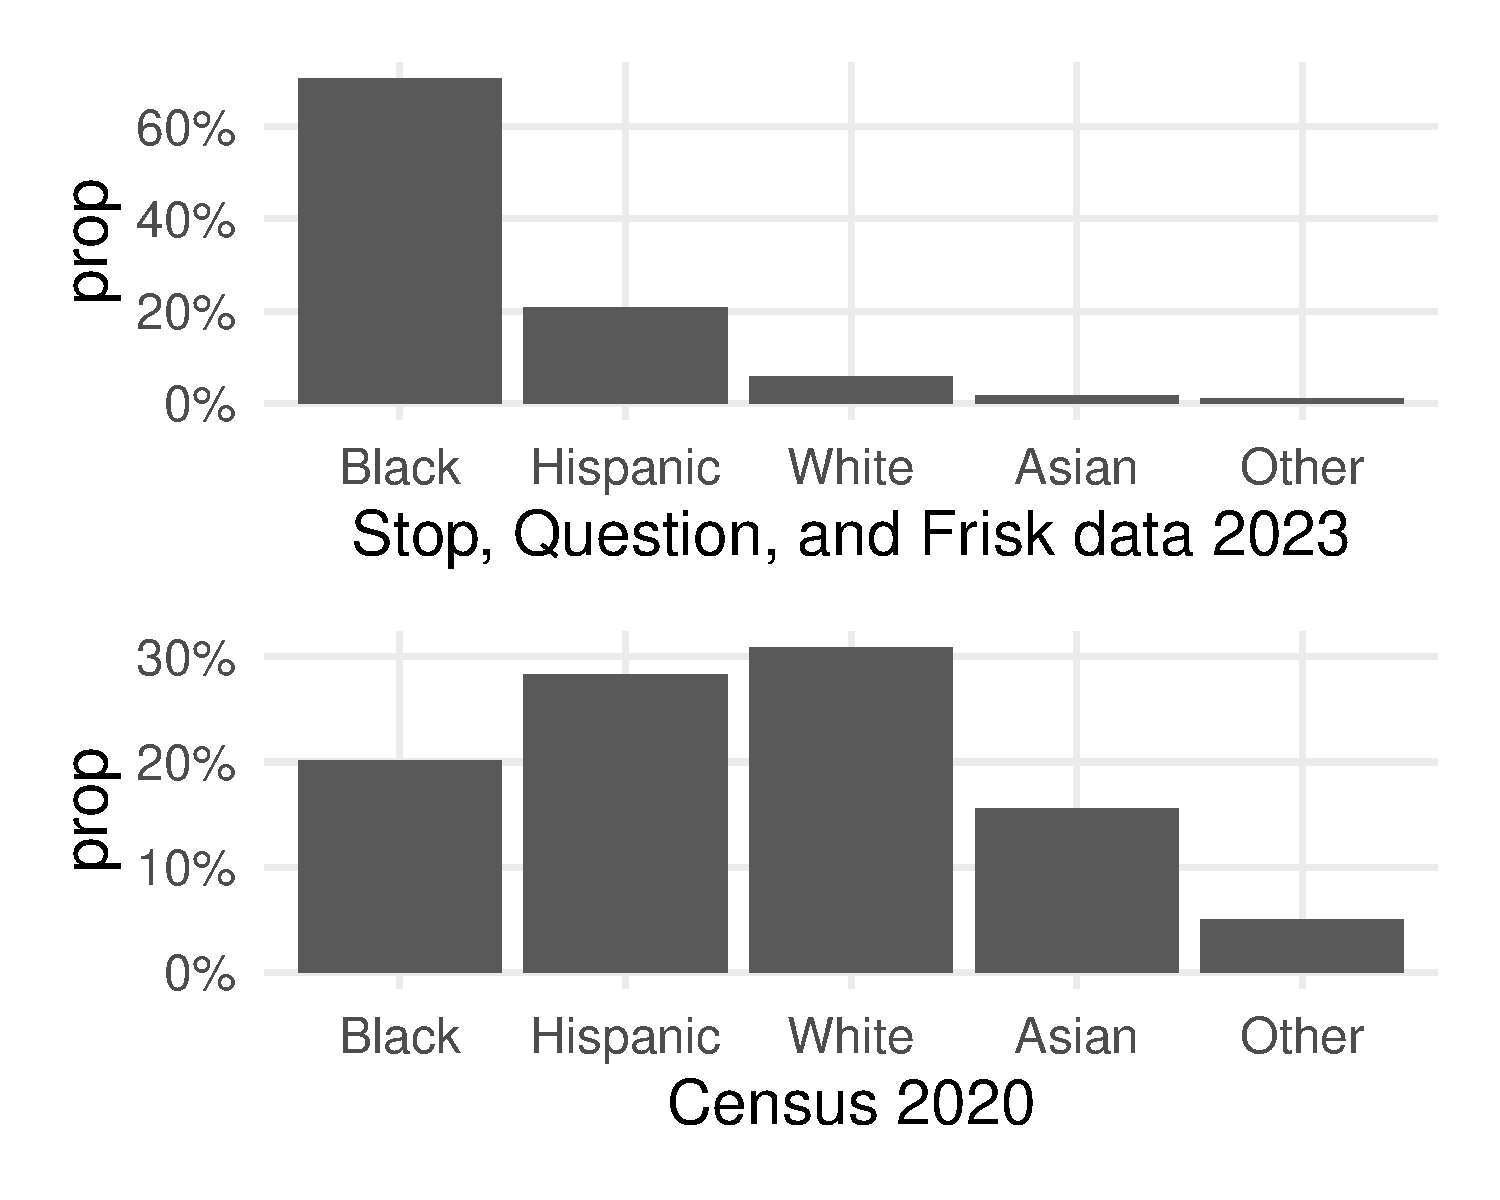
\includegraphics[width=\textwidth]{../figures/sqf_case_study_plot6.pdf}
  \end{minipage}
  \hfill
  \begin{minipage}{0.49\textwidth}
      \centering
      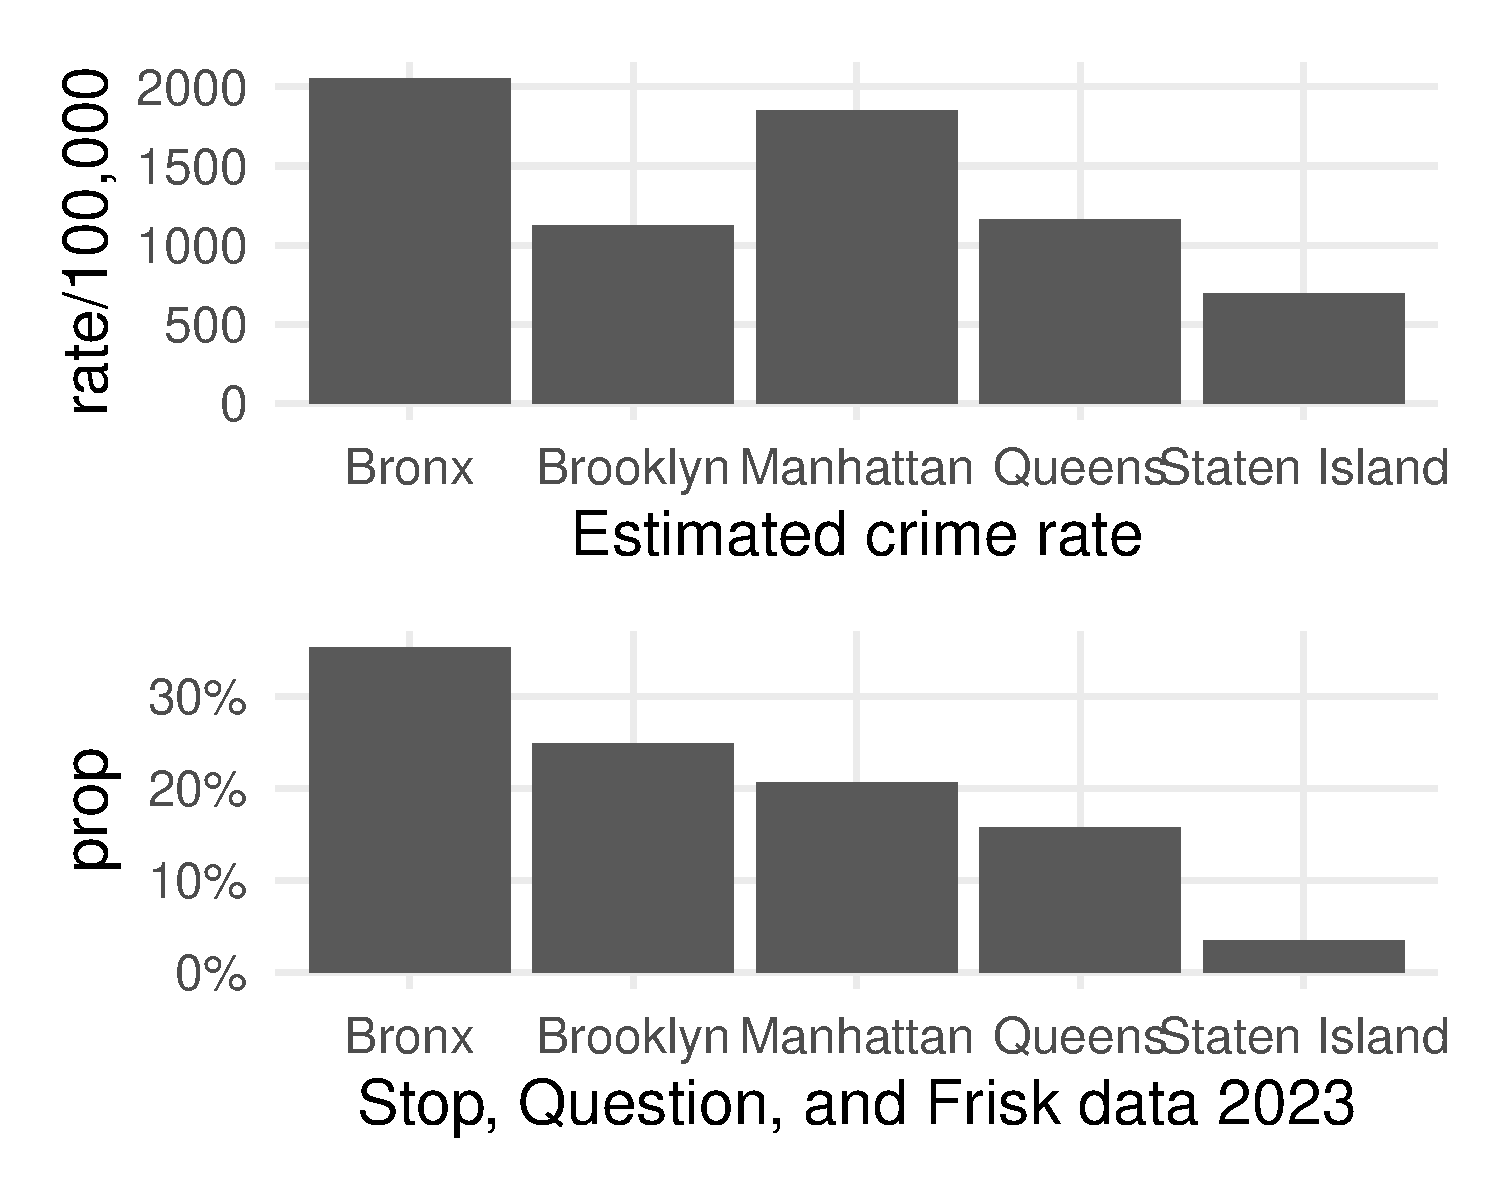
\includegraphics[width=\textwidth]{../figures/sqf_case_study_plot14.pdf}
  \end{minipage}
  \caption{Bar plot comparing the distribution of ethnic groups across boroughs in the SQF 2023 and NYC from 2020 Census (left). On the right a comparison of the estimated borough-wise crime rate per 100,000 citizens with the ethnic distribution of SQF stops.}
  \label{fig:race_distributions}
\end{figure}

As they were the most recent at the time of writing this paper, we work with the stops from 2023. The raw 2023 dataset consists of 16971 observations and 82 variables. We first discarded all the variables that have more than 20\% missing values, which leaves 34 variables.
From this reduced dataset we filter out the complete cases and end up with 12039 observations. \footnote{Simply discarding the missing values and only training on complete cases is discouraged by \cite{fernando2021}. We opt for this approach regardless, since imputation of the missing values is not straight forward
but treating missing values as an extra category will introduce complications when we implement fairness methods.} \\

We summarize "Black Hispanic" and "Black" into the group "Black" and  "American Indian/ Native American" and "Middle Eastern/ Southwest Asian" into the "Other" category. Black people are by far most often stopped, making up 70\% of the total stops; yet, according to 2020 census data black people make up only 20\% of the city's population \autoref{fig:race_distributions}. At the same time white people form the majority of New York citizens (30\%) but contribute with only 6\% to the stops. 
After 2012 there has been a stark decline in stops and the police is known to focus their attention on high crime areas. Therefore, we further look at each borough. 
The most stops in 2023 occur in Bronx and Brooklyn. Based on report of the NYPD and population statistics from 2020, the Bronx also has the highest estimated crime rate per 100,000 citizens. Manhattan is not far behind in crime rate, but has fewer stops. Note that Bronx and Brooklyn happen to be the boroughs with the highest proportion of black citizens \autoref{fig:race_distributions}.\\

  
Given the historical context of stop-and-frisk, the question arises if a classifier trained on data from the unconstitutional period will perform differently.
We choose data from 2011 as it is the year with the most stops. We carry out the same data cleaning steps for the 2011 data as before, starting with 685724 recorded stops and reducing this to 651567 clean observations. Note that these are more than 50 times more stops than in 2023.
The 2011 data has substantially more low-risk stops, only around 6\% of stops result in an arrest. This is a stark contrast to the 31\% in 2023. In the data, the differences in arrestment rate between groups are slightly lower for 2011 and the highest arrestment rate remains to be for the white group.\\

As features, we select variables that should resemble the information that were available to the officer at the time they made the decision to arrest the person. This includes information about the development of the stop, e.g. whether the person was frisked or a summon issued. We assume that all of these constitute "smaller" hits that happen before an officer chooses the most extreme consequence, an arrest. Additionally, we control for factors, such as the time of the stop or whether the officer was wearing a uniform. This selection of features is inspired by \cite{Badr2022DTFANSP}.

\subsection{Results of the Fairness Experiment}
For the training of the classifiers, we dichotomize the race attribute by grouping "Black" and "Hispanic" as people of colour ("PoC") and "White", "Asian", and "Other" as white ("White"). We run a five-fold cross validation and show the results in \autoref{fig:fairness_experiment}. In the bottom right corner we find fair and accurate classifiers. In terms of fairness reweighing and the equalized odds post-processing method perform best. However, the regular random forest classifier comes close to their fairness performance and performs slightly more accurate. Somewhat surprisingly, it does not make any difference for the fairness if the classifier is trained on 2011 or 2023 data.
We examined the model closer and find that due to the low prevalence in the population, a classifier trained on 2011 data primarily suffers from the highly skewed distribution of arrests. The classifier largely predicts the negative label for \textit{anyone} regardless of race, which overshadows potential fairness concerns. The fairness adjusted logistic regression performs worst in terms of accuracy and fairness.
As the picture could change depending on the chosen fairness metric (y-axis), we also tried out other metrics, such as equalised odds or predictive parity. In all cases the regular random forest does not perform worse in terms of fairness but better in terms of accuracy than most fairness adjusted classifiers.
% result plot fairness experiment
\begin{figure}
    \centering
    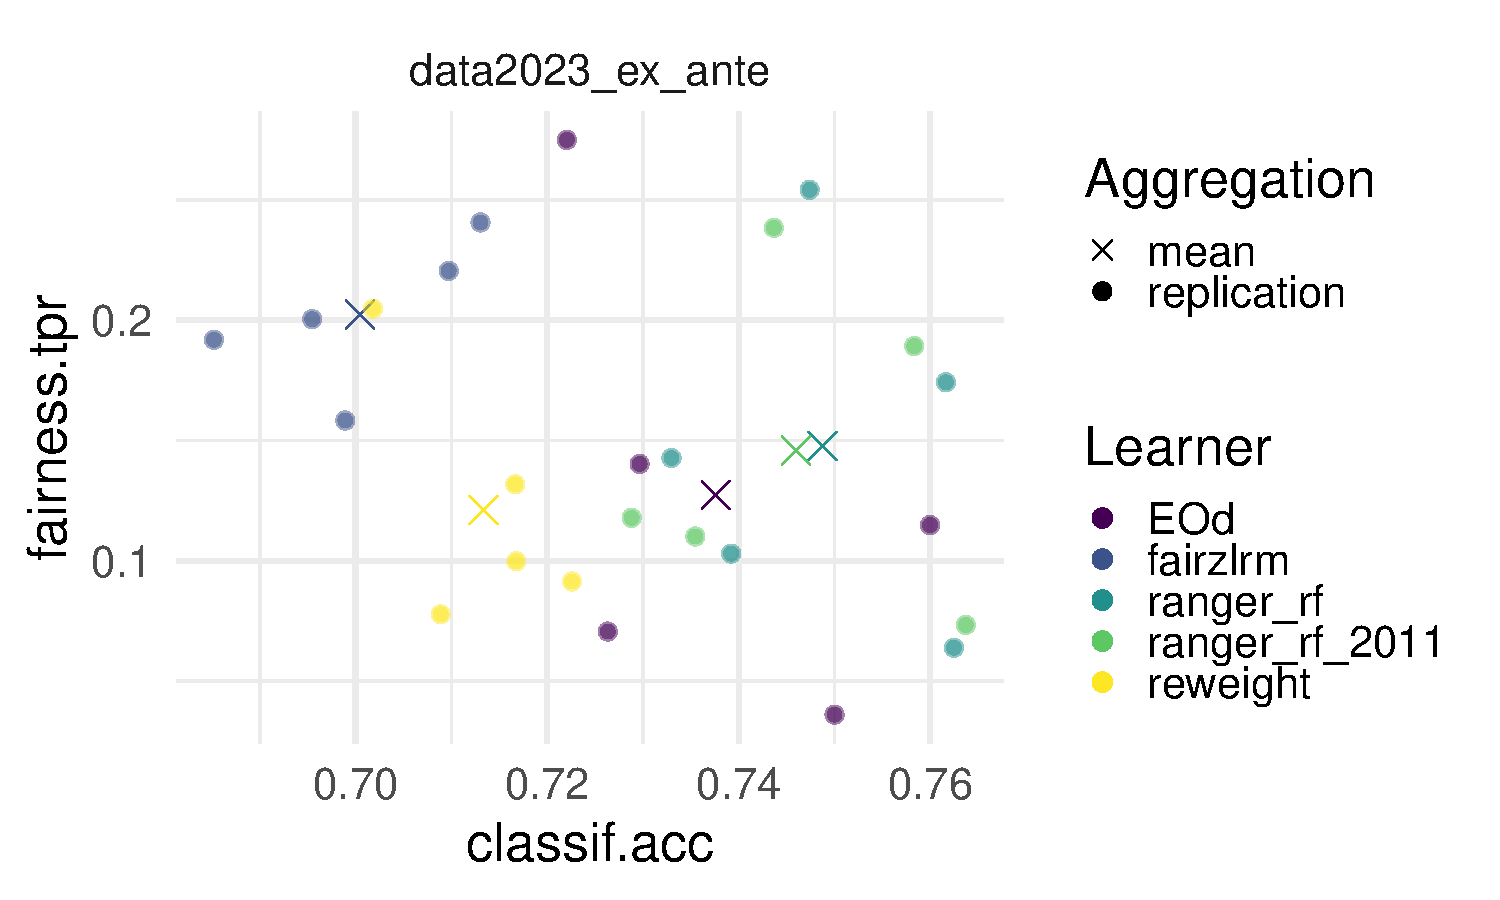
\includegraphics[width=0.7\textwidth]{../figures/sqf_case_study_plot3.pdf}
    \caption{Comparison of learners with respect to classification accuracy (x-axis) and equal opportunity (y-axis) across (dots) and aggregated over (crosses) five folds.}
    \label{fig:fairness_experiment}
\end{figure}

Since the classifiers perform similarly, we choose the regular random forest trained on 2023 to examine the model closer.
On the left we plot the prediction score densities for each group in \autoref{fig:fairness_density}. We can see that in general white people tend to have higher predicted probabilities than PoC. The mode for the scores for non-white individuals is around 0.05 while it is around 0.125 for white individuals. The score resembles the probability of being predicted positive (arrested).
On the right \autoref{fig:fairness_density} we plot the absolute difference in selected group fairness metrics.
Exact equality of the group metrics cannot be expected in practice, so it is common to allow for a margin of error $\epsilon$. Taking $\epsilon = 0.05$, the classifier is fair according to each of the selected metrics, though the difference in positive predictive rates is close to 0.05.
For a more nuanced picture, we additionally report the group-wise error metrics in \autoref{tab:groupwise_metrics_2023}.
The true positive rate, false positive rate, and the accuracy is basically identical between the two groups. So the Separation metrics are fulfilled. More ore less notable differences can only be seen in the Sufficiency metrics: the negative predictive values/ positive predictive value.\\

\begin{figure}
    \centering
    \begin{minipage}{0.49\textwidth}
        \centering
        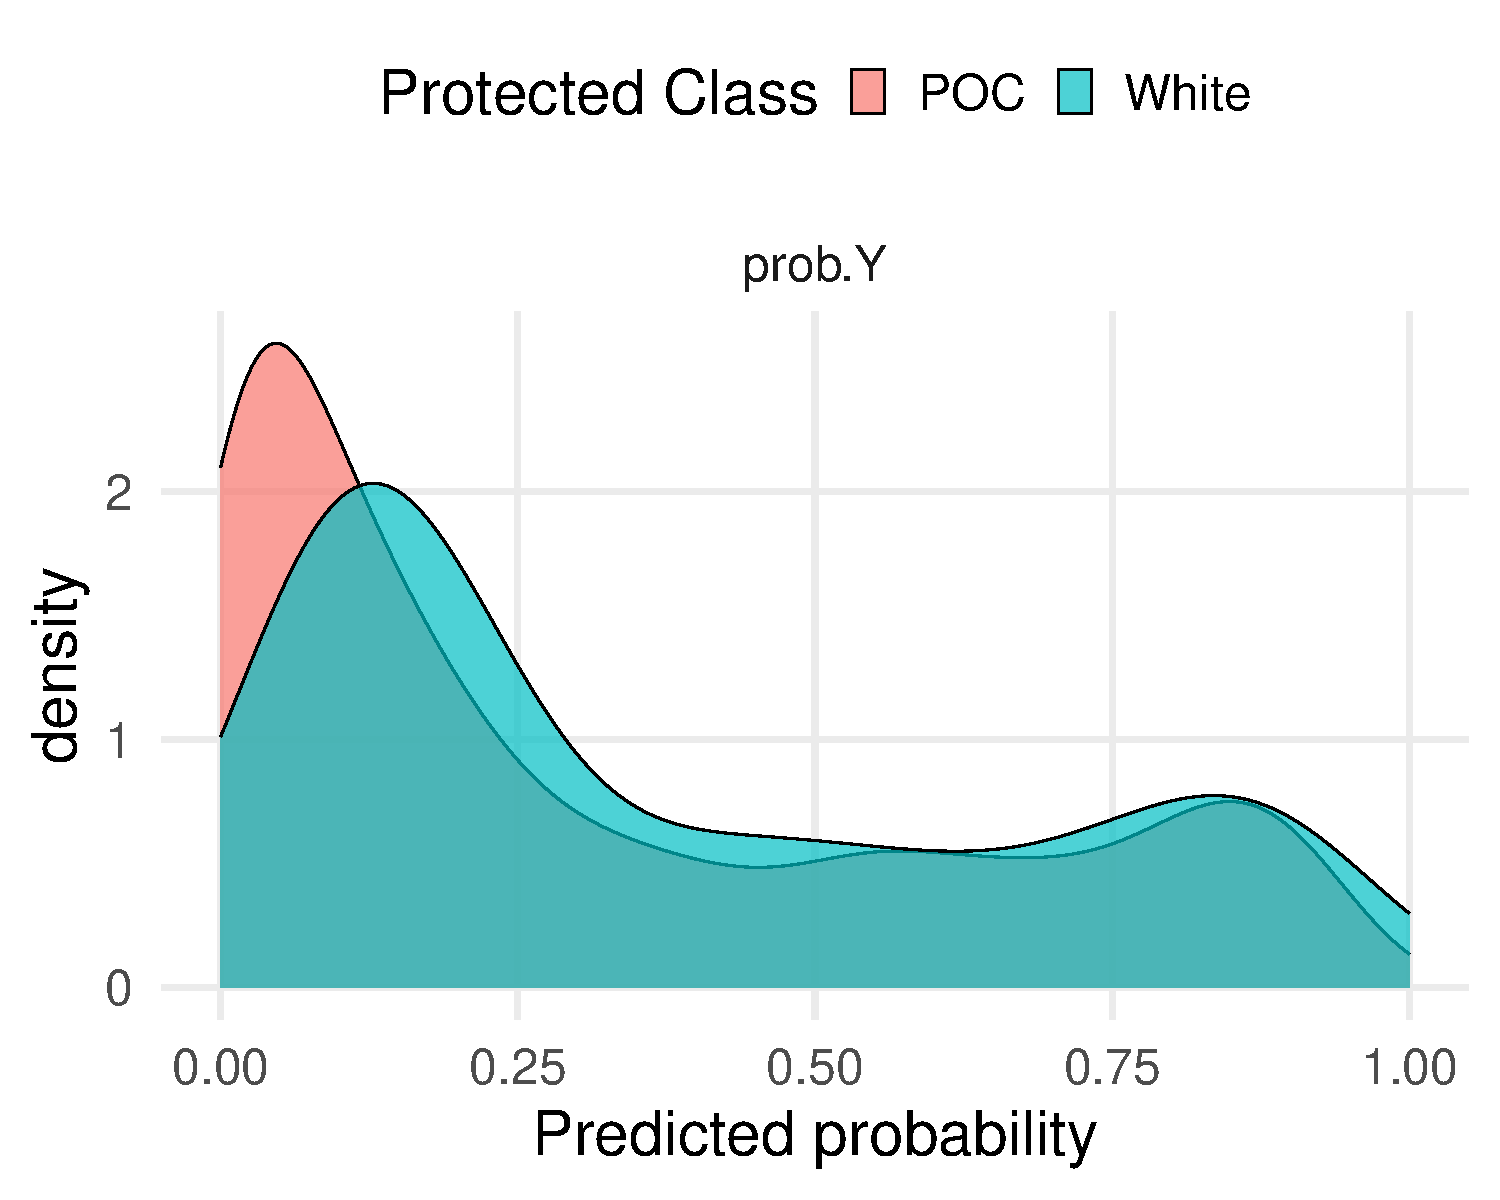
\includegraphics[width=\textwidth]{../figures/sqf_case_study_plot1.pdf}
    \end{minipage}
    \hfill
    \begin{minipage}{0.49\textwidth}
        \centering
        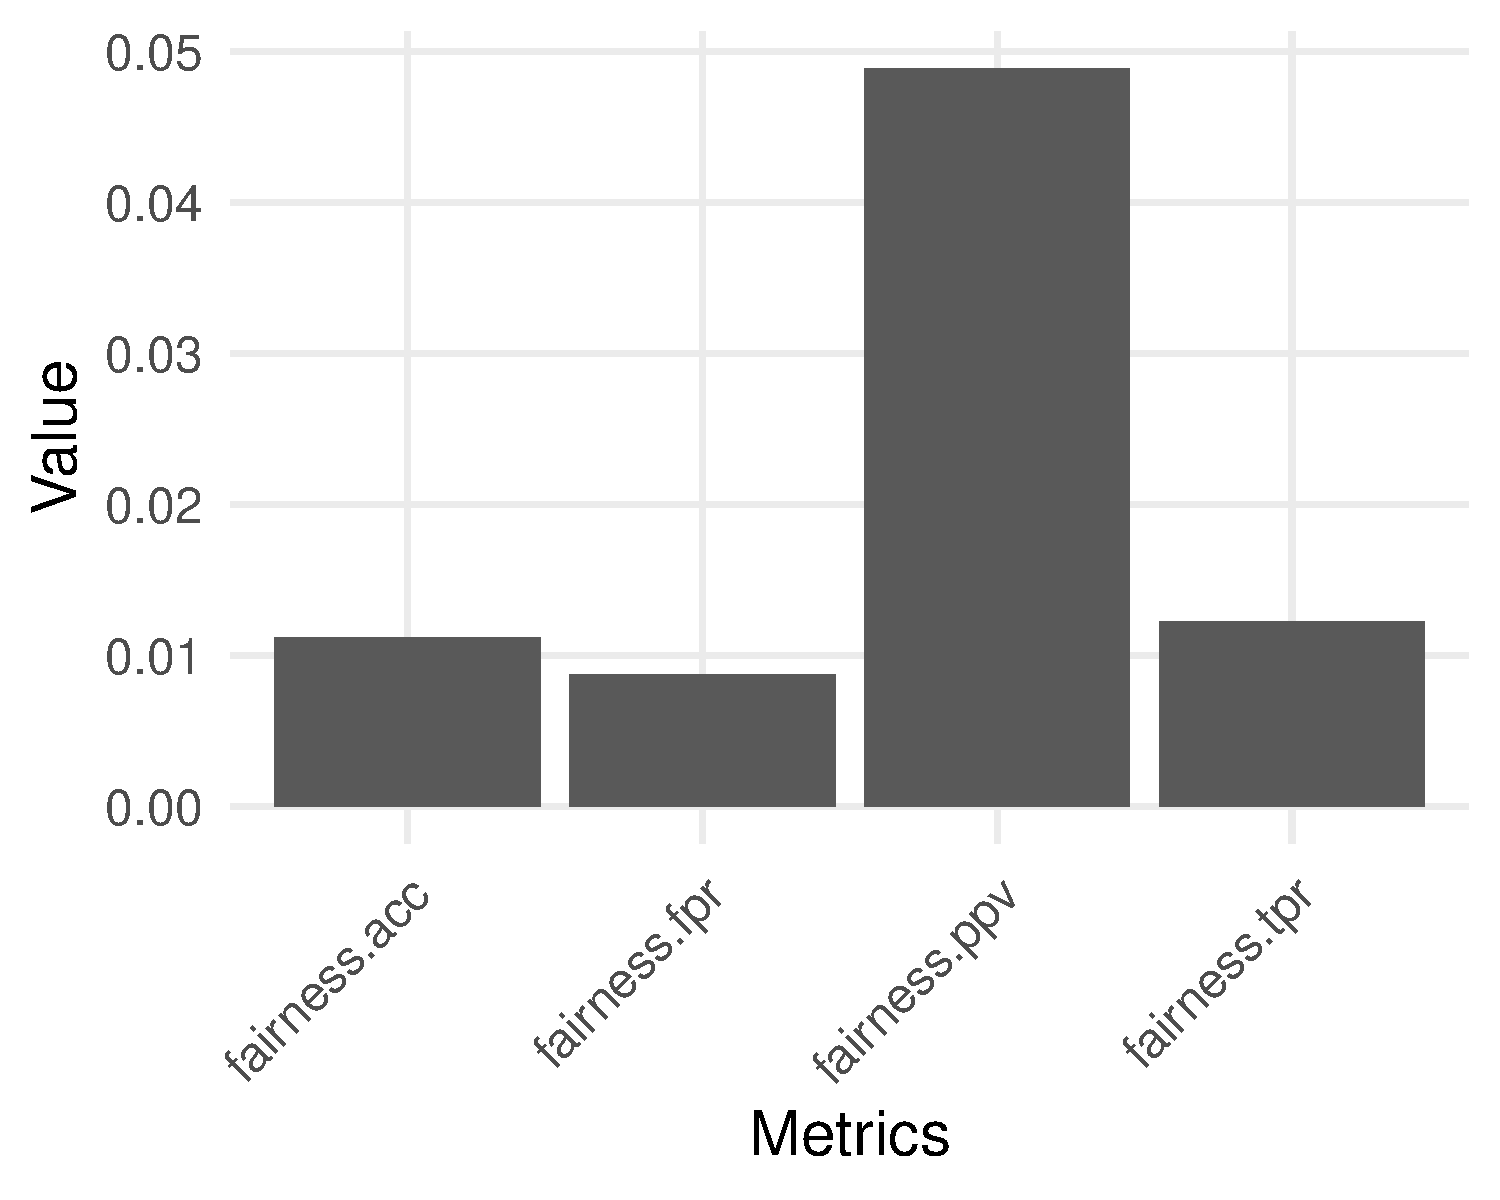
\includegraphics[width=\textwidth]{../figures/sqf_case_study_plot2.pdf}
    \end{minipage}
    \caption{Fairness prediction density plot (left) showing the density of predictions for the positive class split by "PoC" and "White" individuals. The metrics comparison barplot (right) displays the model's absolute differences across the specified metrics.}
    \label{fig:fairness_density}
\end{figure}

% results table
\begin{table}[ht]
  \centering
  \begin{tabular}{rrrrrrr}
    \hline
   & tpr & npv & fpr & ppv & fdr & acc \\ 
    \hline
    PoC & 0.75 & 0.89 & 0.07 & 0.84 & 0.16 & 0.88 \\ 
    White & 0.74 & 0.85 & 0.06 & 0.89 & 0.11 & 0.86 \\ 
     \hline
  \end{tabular}
  \caption{Groupwise Fairness Metrics (2023)} 
  \label{tab:groupwise_metrics_2023}
\end{table}

All in all, it seems like a classifier trained on SQF data to predict the arrest of a suspect is not discriminatory against PoC. In contrast, it even performs better on many of the common performance metrics for PoC than for white people. \cite{Badr2022DTFANSP} have similar findings.\\
In their study they choose six representative machine learning algorithms (Logistic Regression, Random Forest, Extreme Gradient Boost, Gaussian Naïve Bayes, Support Vector Classifier) to predict the arrest of a suspect. Fairness is measured with six different metrics (Balanced Accuracy, Statistical Parity, Equal Opportunity, Disparate Impact, Avg. Odds Difference, Theil Index) and separate analysis are conducted with sex and race as PA.
They compare the fairness of the regular learner to the fairness of learner with a pre-processing method (reweighing) and a post-processing method (Reject Option-based Classifier). All in all, they find that the regular models to not perform worse in terms of fairness than the fairness adjusted models. This leads them to conclude "[...] that there is no-to-less racial bias that is present in the NYPD Stop-and-Frisk dataset concerning colored and Hispanic individuals."
What both of our case studies have in common is that the models were trained on recent data. We trained our model on 2023 stops and \cite{Badr2022DTFANSP} used 2019 stops. Since the judgement of how stop-and-frisk was implemented in NYC in 2013, the number of stops has decreased significantly and citizens are in generally less often stopped. After 2014 the stops have been consistently kept at a low level. 
\cite{Badr2022DTFANSP} see this as explanation for their results and state "The NYPD has taken crucial steps over the past years and significantly reduced racial and genderbased bias in the stops leading to arrests. This conclusion nullifies the common belief that the NYPD Stop-and-Frisk program is biased toward colored and Hispanic individuals." Is this the whole picture?





\section{Studies on the SQF Dataset}
\label{sec:studies}

% \begin{figure}
%     \centering
%     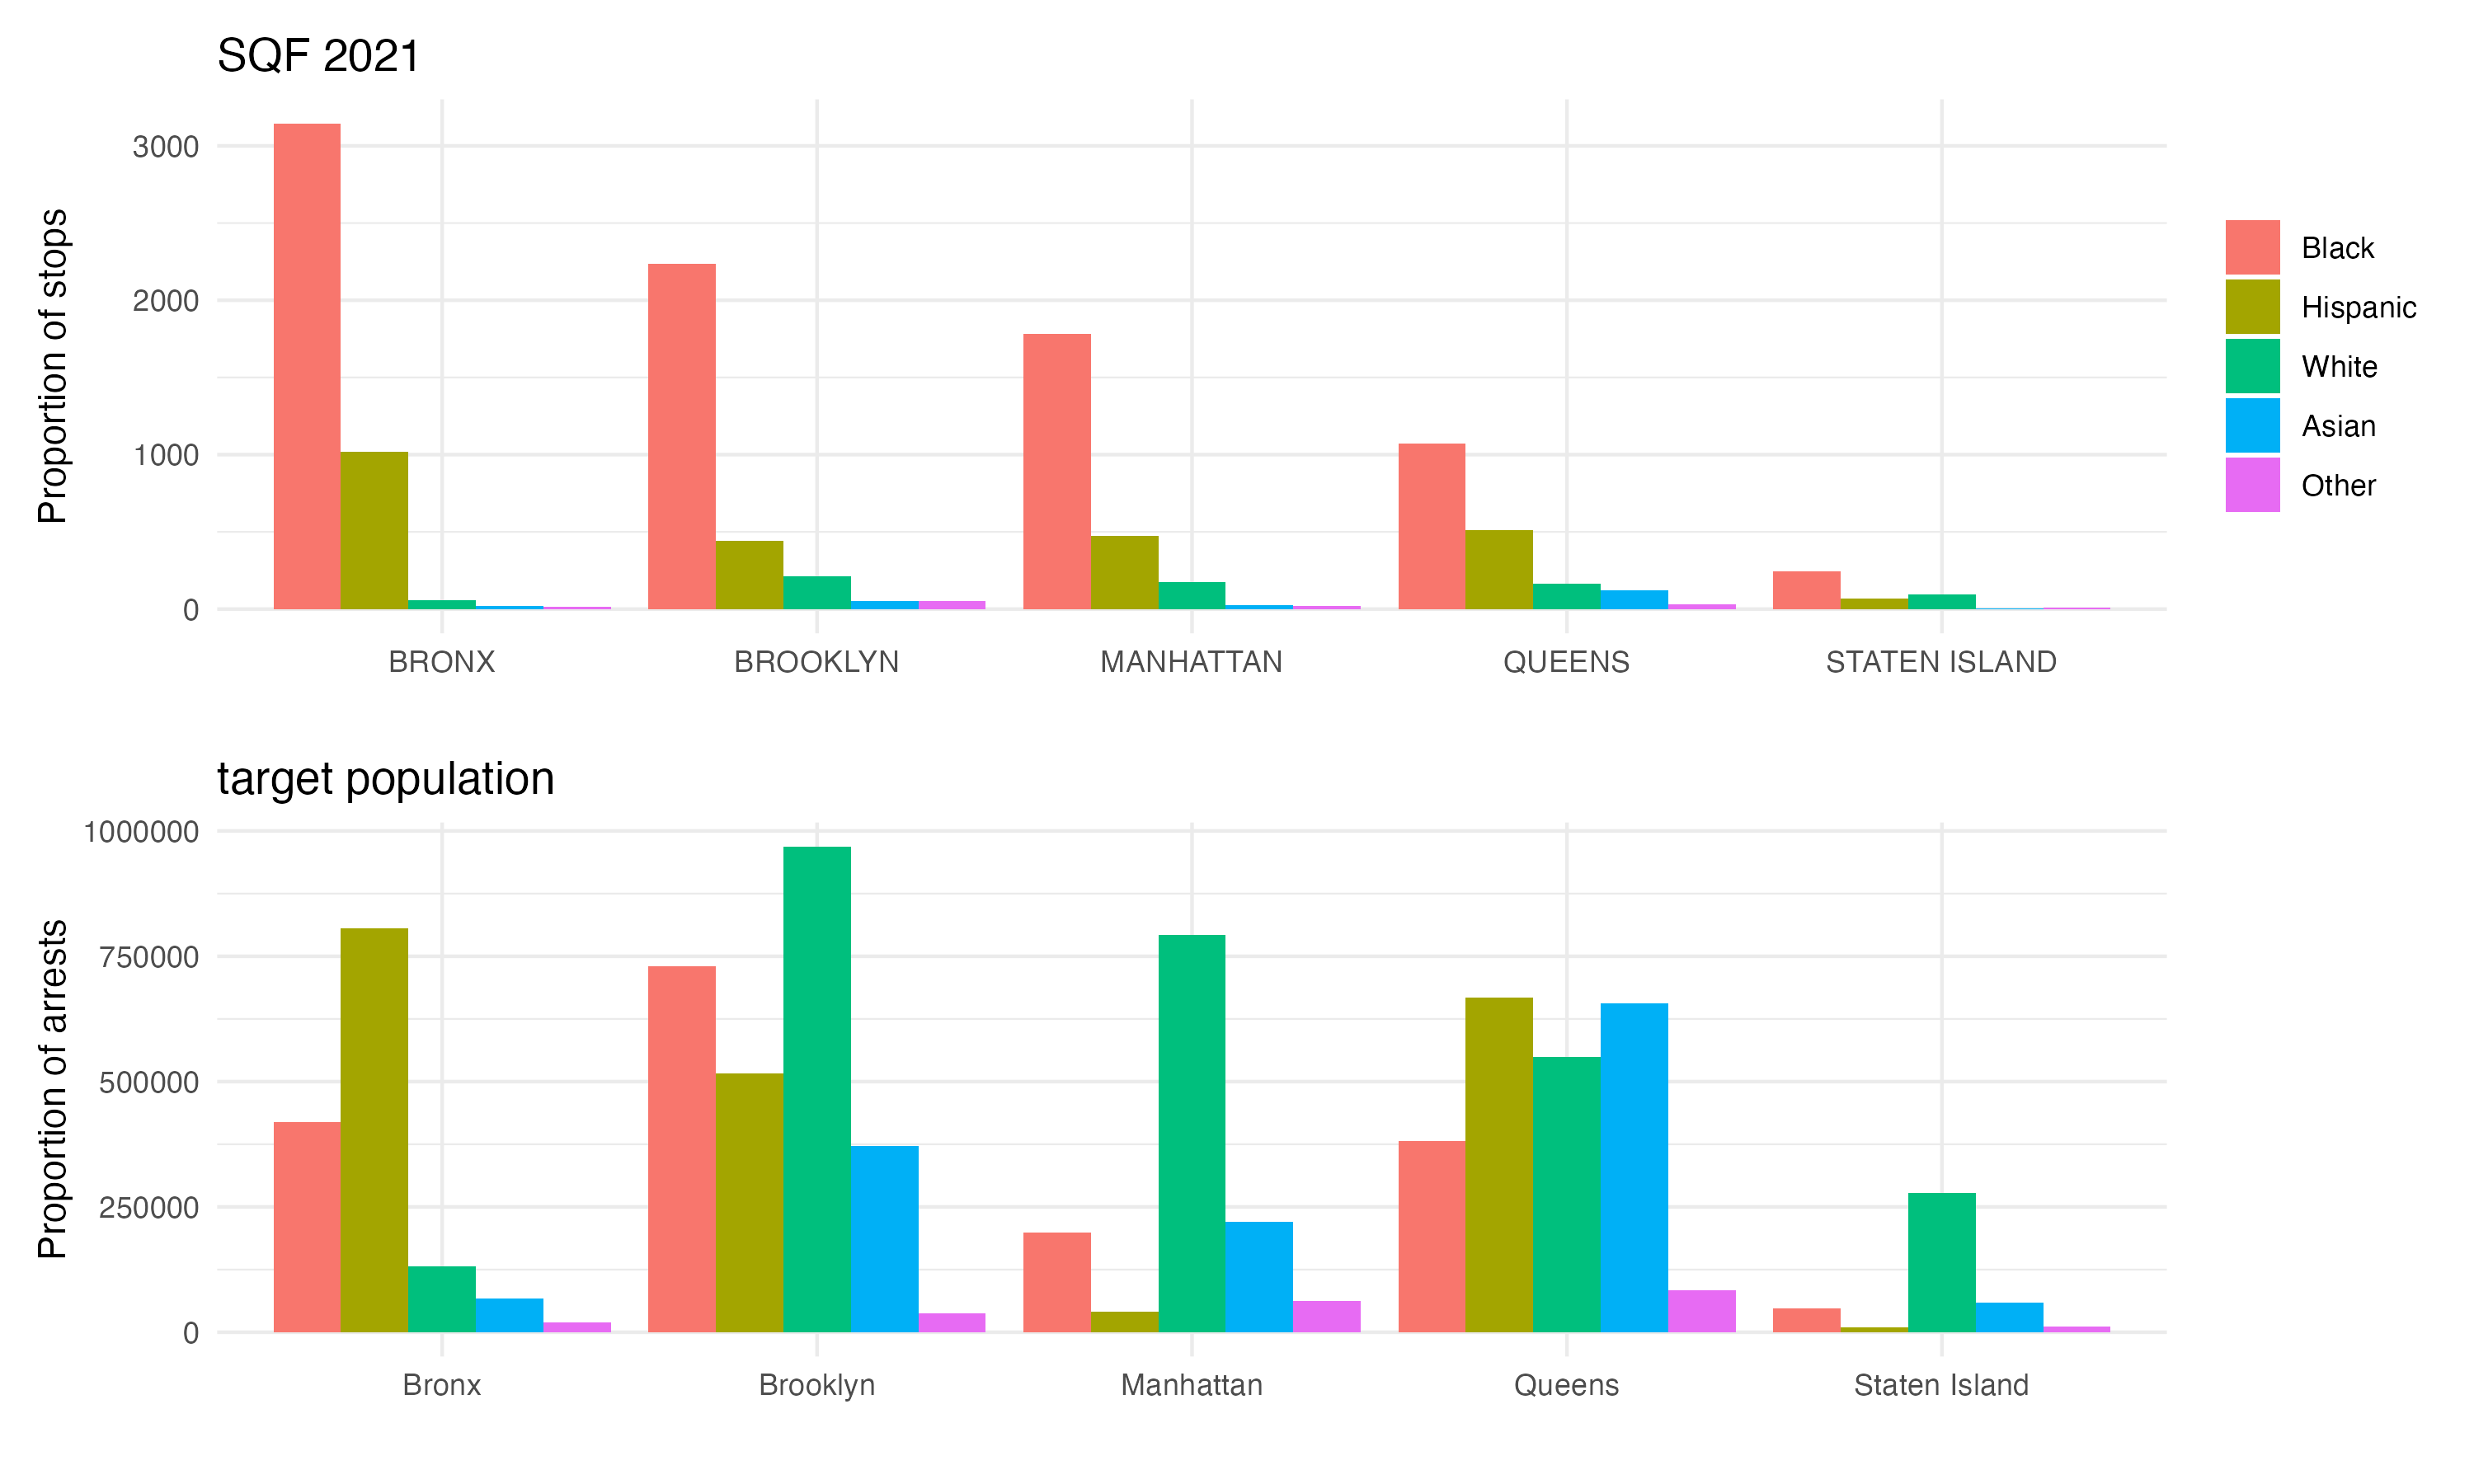
\includegraphics[width=0.7\textwidth]{../figures/sqf_case_study_plot11.png}
%     \caption {Distribution of race by borough in the SQF data (top) and NYC as a whole (bottom).}
%     \label{fig:borough_race_distribution}
% \end{figure}



\subsection{Different approaches to fairness in SQF}

Before going into detail about a specific study, we provide a tabular overview of the different approaches to fairness in the SQF data. We will go into more depth into some of them in the following.

\begin{table}[h]
    \centering
        \begin{tabular}{|m{2cm}|m{3cm}|m{2.5cm}|m{3.5cm}|m{3cm}|}
            \hline
            \textbf{Authors} & \textbf{Task} & \textbf{Model} & \textbf{Fairness Metric} & \textbf{Results} \\
            \hline
            \cite{kallus2018} 
            & Predict prob. of innocence (no weapon) 
            & Log. Regression 
            & Equal Opportunity, Equalized Odds 
            & Bias against PoC \\ 
            \hline
            \cite{RambachanBBOEFW} 
            & Possession of contraband
            & Log. Regression 
            & No explicit fairness metric; evaluate prediction function properties 
            & No bias against PoC\\
            \hline
            \cite{Badr2022DTFANSP} 
            & Predict probability of arrest 
            & Log. Regression, RF, XGBoost, GNB, SVC 
            & Balanced Accuracy, Stat. Parity, Equal Opportunity, Disparate Impact, Theil Index 
            & No bias against PoC \\ 
            \hline
            \cite{Khademi2019FADMELC} 
            & Predict probability of arrest 
            & Weighted regression models
            & FACE causal fairness (group), FACT fairness (individual) 
            & No group bias, but individual bias \\ 
            \hline
            \cite{goel2016} 
            & Predict possession of weapon 
            & (Penalized) Log. Regression 
            & No explicit fairness metric; group-wise hit rates 
            & Bias against Black and Hispanic\\ 
            \hline
        \end{tabular}
        \caption{Summary of SQF-related Fairness Studies}
        \label{tab:sqf_summary}
\end{table}

% \subsection{Sources of bias in the SQF data}
One of the main difficulties that come with the NYPD's data is that, when asking whether stop-and-frisk as a policing strategy is fair, one can come up with various tasks to try to answer this question. Only some of them are suitable to make conclusions about the fairness of the stop-and-frisk policy as a whole.\\
As \cite{Badr2022DTFANSP} we trained a classifier to predict the arrest and used group metrics to assess fairness. Given that both, the 2011 and 2023 regular random forest classifier, performed well on the group metrics, but the stop-and-frisk practice was officially declared unconstitutional for 2011, fairness measured with these metrics for this classification task is not a good indicator for the fairness of the policy as a whole.\\
To answer the question of fairness in stop-and-frisk other studies take a step back and identify a problem with how the data is generated. They formalize and acknowledge that the discrimination in SQF does not solely lie in the outcome of the stop but the decision to stop someone in the first place.

\subsubsection*{Residual unfairness}
\begin{figure}
    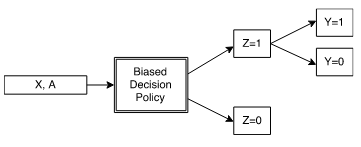
\includegraphics[width=0.7\textwidth]{../figures/selection_bias.png}
    \caption{Selection bias in the SQF data.}
    \label{fig:selection_bias}
\end{figure}

In their paper \textbf{Residual Unfairness in Fair Machine Learning from Prejudice Data} \cite{kallus2018} conceptualize the problem as shown in \autoref{fig:selection_bias}.
A person is defined by their sensitive feature $(A)$ and non-sensitive features $(X)$. For each person in the population of interest a police officer decides whether to stop them $(Z = 1)$ or not $(Z = 0)$. This is the first potential source of bias. It can be seen as a category of selection bias and, referring back to the feedback loop (\autoref{fig:bias_loop}), is introduced by the user.\\
In the SQF context we can imagine that the police is generally more suspicious towards PoC than white people. Alternatively, we can imagine that they are stopping anyone more likely in high crime areas that happen to be mostly low-income neighbourhoods which are largely populated by PoC. \\
Naturally, we can only know the outcome $Y \in \{0, 1\}$ of a stop for the individuals who were stopped. This can create a situation in which the training data produced by the biased decision policy is not be representative for the population the algorithm will be deployed on.\\
\cite{kallus2018} distinguish between target population and training population in such scenarios. The target population is the one on which we want to use the ADM on while the training population are the observations the biased decision policy chose to include in the sample and on which the algorithm is trained.\\
The problem for fairness in this case is that fairness adjustments of the learner (trained on the biased sample) do not translate to the target population. Even fairness-adjusted classifiers can discriminate against the same group that has historically faced discrimination \cite{kallus2018}. They call this remaining disparities in fairness metrics \textbf{residual unfairness}.\\
% The indicator $T \in \{0, 1\}$ tell us whether a person belongs to the target population. If $T = 1$ constantly, it means that the algorithm should be deployed for the entire population of NYC.\\
At this point, we refer back to \autoref{fig:race_distributions}. It shows a clear difference between the racial distribution in the SQF data and the city as a whole. In terms of race, the sample is clearly not representative for NYC\footnote{It can be questioned whether it makes sense to require the SQF sample to be representative for the population of NYC. Does it not make more sense that it should be representative of the population of criminals in NYC?}. At the same time the estimated borough-specific crime rates also differ from the distribution of stops per borough as seen in \autoref{fig:nyc_pop_crimerates_stops_comparison}. \\
They show that their theoretical findings can be observed in the SQF data. Their task is to predict the innocence of a person, while they define innocence based on whether someone carried an illegal weapon (guilty) or not (innocent). The reasoning behind this approach is that the discriminated group is the one that was more often wrongly accused of carrying an illegal weapon. \cite{kallus2018} find that non-white people are indeed wrongfully convicted more often. Even after a post-processing strategy to reach equalized odds, the unfairness against PoC persists as the classifier is used on the target population of NYC as a whole.
% Before an officer stops a person, they need to have a suspicion about what the person did wrong. The suspected crime is recorded in the SQF data. The most common suspicion is the illegal possession of a weapon. \cite{kallus2018} limit themselves to only the stops where the suspected crime of the illegal possession of a weapon. Innocent people can then be defined as the ones, who did not carry a weapon.
% % We refer to \cite{goel2016} for the detailed reasoning behind this approach.
% Note that this is different to \cite{Badr2022DTFANSP} and our analysis, where the arrest is defined as the target variable.\\

% \cite{kallus2018} train a logistic regression classifier and measure fairness in terms of equalized odds and equal opportunity. They find that non-white individuals are more often wrongly accused of possessing a weapon than white individuals. They apply a post-processing technique which assigns group specific thresholds to equalize the false negative rates/true positive rates (and the false positive rates/true negative rates in case of equalized odds) (\cite{hardt2016}).
% After this fairness intervention the error rates are equal between groups when tested on the data the algorithm was trained on. However, when they claim that when the fairness-adjusted algorithm would be deployed on the population of NYC as a whole, racial discrimination against the historically discriminated persists. They do not test their dataset on actual new data from citizens but they design a way to estimate the error rates that would occur when the algorithm is deployed on the target population. They call the unfairness that comes from switching from training population to target population \textbf{residual unfairness} and identify it when training a classifier to predict the possession of a weapon on SQF data.\\
% Here I would need to compare the results of one of the fairness classifiers (probably the EoD post-processing) and compare it to the estimated error rates. Does the classifier inherent the same tendencies?

\subsubsection*{Bias in, bias out?}

% mathematical definitions I really need to get the point across
% - population as tupel of random variables (X, U, A, Y)
% - taste-based discriminator https://link.springer.com/referenceworkentry/10.1007/978-981-33-4016-9_1-1
Another perspective is offered by \cite{RambachanBBOEFW}
While the main message of \cite{kallus2018} is that even fairness adjusted classifiers exhibit the "bias in, bias out" mechanism \cite{RambachanBBOEFW} argue that is depends on the chosen classification task.

% problem setting, intro of selection bias
Similar to \cite{kallus2018} they are interested in whether a person carries a contraband $Y \in \{0, 1\}$. The paper assumes the police is a taste-based classifier against African-Americans. This means they hold some form of prejudice against the group of African-Americans that influences their decision to stop a member of this group. More precisely, they see the biased-decision policy in the decision to search someone $Z = 1$ or not $Z = 0$. Again, only on searched people a contraband can be found. So we are essentially in the same problem setting as before. The goal is to estimate the possession of a contraband $Y$, but we estimate this from $Y | Z = 1$

% They formalise the problem as follows. For the decision-maker (the police) an individual is characterized by the random vector $(X, U, A)$, where X and A have the same meaning as in \cite{kallus2018}
% and U is a set of unobserved features. These latent variables are unknown to the algorithm but are characteristics the police bases their decision to stop someone on. In the SQF context this could be the personal impression the officer got of a suspect which is not recorded and hard to measure.
% In general, for searching any person, an officer incurs a cost $c > 0$. If they search an individual that truly carries a contraband, the officer receives a reward $b = 1$ \footnote{The reward can set to any number b > 0. We assume b = 1 as in \cite{RambachanBBOEFW} without loss of generality.}. In case of searching an innocent person $b = 0$.
% For stopping African Americans the payoff an officer expects increases by $\tau > 0$ compared to stopping a white person. The total payoff for stopping an individual is given by:
% $$Y + \tau * A - c$$
% where $Y$ is the outcome of the search, $\tau$ is the discrimination parameter, $A \in \{0,1\}$, and $c > 0$ is the cost for searching a person.
% Holding the costs $c$ and the outcome of the search $Y$ constant, searching an African American results in a higher payoff than searching a white person. The goal of the police is to maximize their payoff. Therefore, they search an individual according to the following threshold rule:
% $$Z(X, U, R) = 1(E[Y|X, U, A] \ge c - \tau * A)$$
% This means that the threshold for searching an African American is \textit{lower} than for a white person. Consequently, the police searches African Americans more leniently than white people.
% In \cite{RambachanBBOEFW} the authors speak of "selective labels" where again the tupel $(Y, X, A, Z)$ is only available for $Z = 1$. We intentionally used $Z = 1$ to denote the search of an individual as it shows the parallel to the problem setting of \cite{kallus2018} depicted in \autoref{fig:selection_bias}. While in \cite{kallus2018} $Z = 1$ means a person was stopped and therefore included in the sample, in \cite{RambachanBBOEFW} $Z = 1$ means that the person was searched. In the latter study we restrict ourselves to an even smaller subset of the data but the selection bias mechanism remains the same.\\

In contrast to \cite{kallus2018} however argue that the classifier shows the opposite effect; instead of continuing to discriminate the previously disadvantaged group, the classifier exhibits \textit{less} bias as the prejudice against African Americans increases.\\
As the police becomes more biased towards African Americans, they search them more leniently. This means that many innocent African Americans are included in the searched observations. Consequently, the model learns on average lower risk scores for African Americans. Essentially, the data for African Americans becomes more noisy, which lowers the predicted probabilities for this group. The authors call this mechanism \textbf{bias reversal}.\\

As seen in \autoref{tab:sqf_summary} these two studies there are more studies that have worked with the SQF data, each with a unique approach to the question of fairness of the policing strategy. \cite{Khademi2019FADMELC} are also interested in whether the decision to arrest an individual after a stop has been made is discriminatory with respect to race. They design two causal fairness methods, namely the Fair on Average Causal Effect (FACE) and the Fair on Average Causal Effect on the Treated (FACT), to estimate the causal impact of race on the outcome. While one of their metrics finds that the odds of being arrested after a stop are higher for Black-Hispanics than for white individuals, the other metric does not show any racial discrimination.\\
\cite{goel2016} on the other hand focus on the prediction of the possession of a weapon. They find that Black and Hispanic individuals are disproportionately involved in low-risk stops.





% In their second classification task the idea is to train an algorithm to predict whether to search someone in the first place. Now the search becomes the target and here bias inheritance is observed. The same goes for a two stage classification ask that first predicts whether to search and then whether the individual carries a contraband if they were predicted as searched. What happens here is that as more of the stopped African Americans are also searched, the algorithm learns to associate search with more with African Americans than with white people and thus in the future also predicts higher probabilities for a search for African Americans. This is the \textbf{bias inheritance} mechanism.
% We can see parallels to this paper to our own case study in the sense that, PoC indeed have lower risk scores (density plot) and are relatively speaking less often predicted as arrested as white individuals.


% \subsubsection*{Fairness through the lense of causality - problem setting}
% Another paper from the field of fairML by \cite{Khademi2019FADMELC} approached the fairness problem in the SQF data from a causal perspective. As in our case study in section 4 they are interested in whether the decision to arrest someone after they have been stopped is discriminatory with respect to race, while they limit their comparison to Black-Hispanic and White men. They formalize the decision for an arrest made by the officer as a decision function $h: X x A \rightarrow Y$ and estimate the causal effect of race on the outcome from the data. For this they define two causal fairness metrics.
% They write $Y_i^{(a)}$ and $Y_i^{(a')}$ for the outcomes of an observation $i$ when the sensitive attribute $A$ is set to $a$ and $a'$ respectively. Hereby $A = a$ is the observed value of the sensitive attribute for this observation and $A = a'$ is the counterfactual value. In the case of binary PAs this simply means that the person switches group membership. This is relevant because for causal fairness we essentially ask what outcome would the person have had if they were in the other group.\\
% % \begin{definition}
% %     \textbf{Fair on Average Causal Effect (FACE).}  
% %     A decision function \( h \) is said to be fair, on average over all individuals in the population, with respect to \( A \), if  
% %     \[
% %     E[Y_i^{(a)} - Y_i^{(a')}] = 0.
% %     \]
% % \end{definition}

% % \begin{definition}
% %     \textbf{Fair on Average Causal Effect on the Treated (FACT).}
% %     A decision function \( h \) is said to be fair with respect to \( A \), on average over individuals with the same value of \( A \), if  
% %     \[
% %     E[Y_i^{(a)} - Y_i^{(a')} \mid A_i = a] = 0.
% %     \]
% % \end{definition}

% In words, FACE measure the difference between the true prediction and the counterfactual prediction for each data point and averages over these differences. However, in the most extreme case it could happen that $A = black$ were predicted as positive and their counterfactual parts $A = whitee'$ are predicted as negative - so there was a counterfactual switch in predictions. The switch works the other way around for the pairs of (actual white, counterfactual black). This has the consequence that all black individuals get a difference of 1 and all white ones a difference of -1. Taking the average this equalizes and hides the systematic bias.
% This cannot happen with the second definition as we here condition on each group. Averaging out of causal discrimination can theoretically only happen within a group but not between groups anymore. Observational data of course does not contain the information needed for the estimation of their fairness definitions. They use Probability Weighting to estimate FACE and matching to estimate FACT. We refer to \cite{Khademi2019FADMELC} for the details.\\
% To their own surprise, with FACT they find no racial discrimination against Black-Hispanic males, while FACE estimates that Black-Hispanic men are on average more likely to be arrested than white men.



% Overview of SQF studies
% Title: Residual unfairness in Fair Machine Learning from Prejudice Data
% Use of SQF:
% - task: predict probability of innocence (no weapon)
% - model: logistic regression
% - fairness: equal opportunity, equalized odds
% - results: classifier biased towards (Black) Hispanic individuals
% - key concepts: residual unfairness; estimation of error rates in target population via reweighing technique

% Title: Bias in Bias out? Evluating the Folk Wisdom
% Use of SQF:
% - task 1: predict probability of possession of contraband
% - task 2: predict probability of being searched
% - task 3: searched; if searched contraband (two-staged)
% - fairness: no explicit fairness metric; instead properties of the prediction function
% - model: logistic regression
% result: task 1 no discrimination against PoC, task 2 and task 3 discrimination against PoC
% key concepts: bias reversal, bias inheritance

% Title: Data Transparency and Fairness Analysis of the NYPD Stop-and-Frisk Program
% Use of SQF:
% - task: predict probability of arrest
% - model: Logistic Regression, Random Forest, XG Boost, GNB, SVC
%- fairness: Balanced Accuracy, Statistical Parity, Equal Opportunity, Disparate Impact, Avg. Odds Difference, Theil Index
% - results: no discrimination against PoC

% Title: Fairness in Algorithmic Decision Making: An Excursion Through the Lens of Causality
% Use of SQF:
% - task: predict probability of arrest
% - model: weighted regression models (FACE, FACT)
% - fairness: FACE causal group fairness, FACT causal individual fairness
% - results: no group discrimination against PoC, but individual discrimination against PoC
% - key concepts: fair on average causal effect (FACE), f air on average causal effect on the treated (FACT)

% Title: PRECINCT OR PREJUDICE? UNDERSTANDING RACIAL DISPARITIES IN NEW YORK CITY’S STOP-AND-FRISK POLICY
% Use of SQF:
% - task: predict probability possession of weapon
% - model: (penalized) logistic regression
% - fairness: no explicit fairness metric; group-wise hit rates
% - results: Black and Hispanic disproportionally involved in low-risk stops

% formal problem setting
% The selection bias we face means that we only have knowledge about $X, A, Y | Z = 1$ while we do not know $X, A, Y | Z = 0$. All information about the stop, the demographic details of the person and the outcome which serve as training label for an algorithm are only observed for stopped individuals.

% % Fairness definition
% The paper defines fairness via equal opportunity. Equal opportunity demands that the true positive rates across groups are equal, so that truly arrested individuals are predicted as such. In our case, in which a positive prediction $\hat{Y} = 1$ is undesirable it makes more sense to look at the false positive rates (or equivilantely at the true negative rates) and define fairness via predictive equality, i.e. $P(\hat{Y} = 1 | Y = 0, A = a) = P(\hat{Y} = 1 | Y = 0, A = b)$ or $P(\hat{Y} = 0 | Y = 0, A = a) = P(\hat{Y} = 0 | Y = 0, A = b)$.
% The paper looks at a thresholding classifier, if the prediction score exceeds a certain threshold the positive value for the target is predicted.
% This allows us express the false positive rate and the true negative rate of a group $a$ with respect to an event $E$ via the cummulative distibution function. $F_a^E = P(\hat{R} \leq \theta | Y = 1, A = a, E)$. Note that we condition on the truly negative subject in the sample. In the SQF case this would mean that we only look at people that were innocent, so not arrested.
% The truly arrested that have a predicted probability $\hat{R} \leq \theta$ are wrongly classified as not-arrested, while the ones for whom $\hat{R} > \theta$ are correctly classified as arrested. $F_a^Z$ gives us nothing other than the false negative rate in the training population and $F_a^T$ is the false negative rate in the target population.
% When we want to define a predictive equality classifier on the training population we require $F_a^Z(\theta_a) = F_b^Z(\theta_b)$ to hold. 

% % Definition of fair classifier 
% An optimal derived predictive equality classifier can then be defined as $\hat{Y} = I(\hat{R} > \theta_A)$ and $F_a^Z(\theta_a) = F_b^Z(\theta_b)$ for all groups a,b. In words, the classifier predicts the positive (undesirable)  outcome with a group-specific threshold for each member of the group while this group specific threshold is set in such a way that predictive equality on the training data is fulfilled. We will not go into detail of how one finds such a classifier but refer to \cite{hardt2016} who propose a post-processing method to derive the optimal thresholds for each group. 

% % Definition of unfairness inequity of predictive equality
% With the definition of fairness as predictive equality (equal tnr/fpr across groups) we can in turn define unfairness as nothing other than the difference in true negative rates between groups, i.e. \(\epsilon_{a,b}^E = P(\hat{Y} = 0 | Y = 0, A = a, E) - P(\hat{Y} = 0 | Y = 0, A = b, E)\) and call this inequity of predictive equality. $\epsilon_{a,b}^{T=1} > 0$ shows discrimination against group b, since this means that the true negative rate for group b is lower than for group a.
% When we construct an equal opportunity classifier (via some fairness intervention) then $\epsilon_{a,b}^{Z=1} = 0$ holds for this classifier. This also means that any unfairness that might show in the target population cannot be explained via existing ineuqities between groups in the training population but via existing differences in the training and the target population. So it is unfairness that gets introduced when we try to generalize our algorithm to the population it was not trained on. \cite{kallus2018} call this residual unfairness, since this is unfairness remaining event after fairness adjustments.

% % Scenarios of discrimination
% \subsubsection*{Strong disparate benefit of the doubt}
% To fully understand the results of the paper, we additionally introduce the concept of stochastic dominance, originating from decision theory. Let $F, G$ be two cummulative distribution functions. Then $G$ first order stochastically dominates $F \preceq G$ when $F(\theta) \geq G(\theta)$ $\forall\theta$. Recall that G and F are cumulative distribution functions. So first order stochastic dominance of G over F, smaller values of G for each input value $\theta$, that the population described by the CDF of G consistently has higher probability values than population F. Their probability mass is concentrated towards the higher input values thus the cummulative distribution function is small for small input values.
% Equipped with these definitions the paper constructs difference scenarios of (un)fairness. The bottom line is always that equal opportunity in the training population does not guarantee equal opportunity in the target population. We will introduce the one scenario mathemtically aligning the statements of the paper with the sqf scenario and will only conceptually explain the oterh scenarios which are extensions of the first one.

% % Scenario 1: Strong disparat benefit of the doubt (Prop. 2)
% We assume the following:
% $F_a^{Z=1} \succeq F_a^{T=1} and F_b^{Z=1} \preceq F_b^{T=1}$ and at least one of the equalities does not hold (either $F_a^{Z=1} \ne F_a^{T=1}$ or $F_b^{Z=1} \ne F_b^{T=1}$ or both).
% Then every derived equal opportunity classifier has nonnegative inequity of predictive equality for group b relative to group a $\epsilon_{a,b}^{T=1} \geq 0$ and at least one derived equal opportunity classifier will have a strictly positive inequity of predictive equality disadvantaging group b relative to group a $\epsilon_{a,b}^{T=1} > 0$.

% In words this means that for group a in the training population we have way more people with high scores (propbabilities of getting positive (undesirable) prediction) than in group a of the target population.
% So group a members were stopped very carefully. For group b members the opposite is true. In the train population of group b, there are many more people with low risk scores than there are in the target population of group b. This means group b members were stopped very leniently. 
% This aligns with the fact that the sqf data records considerably more stops for black people than white people. In this case the propositions of the paper will show us again that even after adjusting for equal error rates, the classifier will disadvantage group b when applied to the target population.
% The results of the paper would then say that adjusting a classifier for predictive equality, so equal false positive rates across groups, is not enough to ensure fairness on a whole and in future application. 

% % Extentions of scenario 1
% The paper admits that the assumptions are strict and in reality unlikeliky to be met. The assumptions would mean that the police is so biased against group b members that the proportion of low-risk group b members among stopped individuals is higher than the proportion of low-risk gorup b members in the general population. This would require a very unreasonable stopping policy.
% Therefore in the propositions that follow they weaken the assumptions. They allow that the stochastic dominance works in the same direction for both groups but the difference in training and target population for group b is so much more different than for group a that discrimination persists.
% Recall that the fairness definition of the paper is based on true positive rates and they are especially interested in the post-processing method by Hardt et al. The method takes as input the error rates of a classifier (e.g. the false positive and true positve error rates) in order to find group-specific thresholds that equalise these error rates across groups.
% If we now put in the "wrong" error rates, the error rates of the training population, which, however, are nto representative for the target population due to selection bias, we estimate the wrond thresholds. Therefore Kallus and Zhou offer a way to estimate the error rates in the target population based on training data and some additional information.
% These "corrected" error rates can then be used to create fairness interventions that will also spill over to the target population. Their approach is interesting and they use it on the SQF data themselves, but it is also very tailored towards error-rate-based group metrics and is mostly useful when the fairness method relies on the error rates, such as the thresholding by Hardt et al. When the fairness methods does not take error rates as an input, there is little use in estimating them for the target population.
% Though it could be interesting regardless, to get picture for how the algortihm could generalise.

% As the fairness audit in the previous chapter showed little disparities, we only take their method to estiamte the generalisation of the algorithm.
% We match the target population to the training population via borough.


% Things I have to introduce when I want to presente the math of the paper (e.g.Preposition 2)
% - Stochastic dominance
% - derived equal opportunity classifier
% - inequity of opportunity (epsilon)
% - Fairness defintion (equal tnr; predictive equality)
% \section*{Bias in, bias out - an alternative perspective}

% mathematical definitions I really need to get the point across
% - population as tupel of random variables (X, U, A, Y)
% - taste-based discriminator https://link.springer.com/referenceworkentry/10.1007/978-981-33-4016-9_1-1

An interesting perspective on this observation can be found in \cite{RambachanBBOEFW}. They take a different stance on the problem of biased training data than \cite{kallus} and question the "bias in, bias out" mechanism.

They formalise the problem as follows. For the decision-maker (the police) an individual is characterised by the random vector $(X, U, A)$, where X and A have the same meaning as in \cite{kallus}
and U is a set of unobserved features. These latent variables are unknown to the algorithm but are characteristics the police bases their decision to stop someone on. In the SQF context this could be the personal impression the officer got of a suspect which is not recorded and hard to measure.

The paper assumes the police is a taste-based classifier against African-Americans. This means they hold some form of prejudice against the group of African-Americans that influences their decision to stop a member of this group.
In general, for stopping any person, an officer incurs a cost c > 0. If they stop an individual that turns out to be involved in criminal activity and is therefore arrested, the officer receives a reward b = 1 \footnote{The reward can set to any number b > 0. We assume b = 1 as in \cite{RambachanBBOEFW} without loss of generality.}. In case of stopping an innocent person b = 0.
For stopping African Americans the payoff an officer expects increases by $\tau > 0$ compared to stopping a white person. The total payoff for stopping an individual is given by:
$$Y + \tau * A - c$$
where $Y$ is the outcome of the stop, $\tau$ is the discrimination parameter, $A \in \{0,1\}$, and $c > 0$ is the cost for stopping a person.
Holding the costs $c$ and the outcome of the stop $Y$ constant, searching an African American results in a higher payoff than searching a white person. The goal of the police is to maximise their payoff. Therefore they stop an individual according to the following threshold rule:
$$Z(X, U, R) = 1(E[Y|X, U, A] \ge c - \tau * A)$$
This means that the threshold for stopping an African American is \textit{lower} than for stopping a white person. Consequently, the police stops African Americans more leniently than white people.
This taste-based discrimination rule is the biased decision policy introduced in \cite{kallus}. In \cite{RambachanBBOEFW} the authors speak of "selective labels" where again the tupel $(Y, X, A, Z)$ is only available for $Z = 1$. 

In short: It actually depends on the outcome and the training sample whether the discrminiation of the previously discriminated (bias interhitance) exists. In some cases it can actuall come to the opposite effect, which they call bias reversal.
The mechanism is as follows: the historically discriminated groups is very represented in the sample as being included is an act of discrimination itself. This means we have more training data for the disadvantaged group, they resemble the target population more, as they were more leniently included, and thus the classifier generalised better to the disadvanteged group.
When we collect more data for the group, we come closer to the target population and our classifier will work better on the target population for the group with more data.


Black people are more leniently stopped, leading to higher stopping rates in for black people in the training data, meaning
more training data for this group. Because we stop black peopel more leniently, we record many innocent black people in our data.
In \cite{kallus} this would lead to a lower learned threshold \footnote{first this leads to lower risk scores for black individuals. And then via fairness adjustments (e.g. for equalized odds) this leads to lower thresholds for black individuals.}
for black individuals. Applied on the target population this would mean that we would predict too many false positive. The threshold estimated from the training 
data is so low that we classify to many people as guilty because in the target populations the scores are actually higher and meet the threshold easily.
In \cite{RambachanBBOEFW} they say that by stopping (searching, they actually talk about searching, not stopping) black people so leniently, our sample for black people comes actually pretty
close to the target population.
In other words, the training data for black people is pretty close to the target data for black people, which means that our classifier will work well on the
target population for black people. \\
To summarise, in \cite{kallus} bias against a group results in a less representative sample. In \cite{RambachanBBOEFW} bias against a group results in a more representative sample.


\textbf{Theorem 1}\\
The prediction for african americans is weakly decreasing in tau. This means, as tau increases (so racial bias increases), the expected value for Y gets actually lower,
so closer to zero, so less often predicted to have a contraband. What is happening? Higher tau means lower searching threshold for african americans.
So the data for african americans becomes "more noisy", more and more innocent people come into our sample, so we predict lower risk for african americans. 
In \cite{RambachanBBOEFW} paper this translates to a more representative training data for african americans and thus also better performance on the general population of african americans.
In \cite{kallus} paper the mechanisms is the same, we also estimate lower risks cores for african americans, but then sth else happens.
I think in Kallus we then do a fairness intervention that leads us to setting a LOWER threshold for african americans, meaning we predict them as
guilty more easily to achieve the same FPR as in the other group. I think in kallus they first formulate it in the strict way, where the police is so biased against african americans
that the stopped african americans are LESS likely to actually have a weapon than the general population. But they relax this setting afterwards.


What happens if we train the logistic classifier (to predict weapon yes no) on the SQF as is (Kallus), don’t do a post processing fairness intervention (NO Hardt et. al)
and test the classifier on the target population (that is created via the weighing method of Kallus and Zhou)? I think according to \cite{RambachanBBOEFW} we should observe bias reversal.

\section{Conclusion}

More concrete limitations and what future work could adress. Be as conrete as possible.
Limitations of our own case study:
- we followed principle of \cite{Badr2022DTFANSP} ans just as them did not find any unfairness; taking the findings from a classifier trained to predict arrest and make conclusions about the fairness of SQF practice as a whole is a big jump.
- we only trained on 2023 or 2011 data separately but did not take years together; other studies took multiple years; due too limited resources had to keep computation time low

Interesting to explore from here:


In conclusion, the questions of fairness for SQF is difficult.
Before any fairness intervention, we have to formulate a clear fairness question. It is something entirely different to ask if the stop, question, and frisk practice (as a whole) is fair or whether a classifier to predict the arrest of a person trained on SQF data is fair? Or whether a classifier trained to predict the possession of a weapon trained on SQF data is fair?
The exact question we formulate leads us to look at different aspects of the data. In this paper we got a first idea of the answer to the first questions by comparing certain characteristics of the SQF population to the population of NYC as a whole (descriptive analysis) and find that the two populations do differ. But does it make sense to want the SQF sample be representative for whole NYC or does it not make more sense to want it to be representative of the population of criminals in NYC?
Here we see a closer match in racial distributions. This, however, is by far not enough to claim the fairness of the police practice. Crime statistics have to be read with caution. They are influenced by many factors, including the amount of police in a certain area, the socio-economic status of the population and the trust in the police. Historical discrimination leads to lower socio-economic, lower socio-economic status comes with higher crime rates, higher crime rates lead to more police in the area, more police in the area lead to more reported crime. Crime statistics are embedded in a broad context and do not necesarily reflect objective inherent truths but our social and economic system.
We can cite \cite{goel2016} who approach the question in a more wholistic way, account for complex factors and come to the conclusion that SQF is over-targetting PoC.
As we saw in our own case study and \cite{Badr2022DTFANSP} also find, is that this does not mean a classifier trained on SQF data violates group fairness. Depending on the task some classifiers might perform better on the historically disadvantaged group while others in fact discriminate against them.
With this study we do not claim to give the answer to fairness in SQF but the goal was to show the readers the complexity of the situation/ give critical perspective/ show different approaches to fairness in SQF. As many datasets, this one comes with a great backstory (socio-economic context, historical biases) and problems (group imbalance, ...) and all of this is entangled. We should be aware of this otherwise it might misinterpretation of results.



\newpage

% \includeonly{chapters/introduction.tex, chapters/results.tex}
% include{}

% \section{Data}
% \label{Data}
% \input{Chapter/Data.tex}
% \newpage
\newpage

% ------------------------------------------------------------------------------
% listoffigures ----------------------------------------------------------------
% ------------------------------------------------------------------------------

% \setcounter{page}{3} % CHANGE

\listoffigures
% \input{Chapter/List of figures.tex}

% ------------------------------------------------------------------------------
% listoftables -----------------------------------------------------------------
% ------------------------------------------------------------------------------

\listoftables
% \input{Chapter/List of tables.tex}


% ------------------------------------------------------------------------------
% APPENDIX ---------------------------------------------------------------------
% ------------------------------------------------------------------------------
    
\pagenumbering{Roman}

\setcounter{page}{5} % CHANGE

\appendix

% \section{Appendix}
% \label{app}
% \input{Chapter/Appendix A.tex}
% \newpage

\section{Electronic Appendix}
\label{el_app}
See the GitHub repository for data, code and illustrations:
\href{https://github.com/juliet-fleischer/SQF_fairness_project}{SQF Fairness Project}
\newpage

% \input{Chapter/Appendix B.tex}
% \newpage

% ------------------------------------------------------------------------------
% BIBLIOGRAPHY -----------------------------------------------------------------
% ------------------------------------------------------------------------------

\RaggedRight
% \bibliography{../literature.bib}
% \bibliographystyle{dcu}
\printbibliography
\newpage
% ------------------------------------------------------------------------------
% DECLARATION OF AUTHORSHIP-----------------------------------------------------
% ------------------------------------------------------------------------------
\Large
\noindent
\textbf{Declaration of authorship} 
\vspace{0.5cm}
\noindent
\normalsize

I hereby declare that the report submitted is my own unaided work. All direct 
or indirect sources used are acknowledged as references. I am aware that the 
Thesis in digital form can be examined for the use of unauthorized aid and in 
order to determine whether the report as a whole or parts incorporated in it may 
be deemed as plagiarism. For the comparison of my work with existing sources I 
agree that it shall be entered in a database where it shall also remain after 
examination, to enable comparison with future Theses submitted. Further rights 
of reproduction and usage, however, are not granted here. This paper was not 
previously presented to another examination board and has not been published.
\\

\vspace{1cm}
\textcolor{orange}{Munich, \mydate} \\

\vspace{3cm}

\noindent\rule{0.5\textwidth}{0.4pt} \\

\textcolor{orange}{\myname}

\end{document}
